\documentclass[UTF8,zihao=-4,openany,fontset=fandol]{ctexbook}

\usepackage[a4paper,top=2.4cm,bottom=2.4cm,left=2.6cm,right=2.6cm,headheight=15pt]{geometry}
\usepackage{amsmath,amssymb,bm,mathtools}
\usepackage{booktabs,longtable,tabularx,array,multirow}
\usepackage{graphicx,float,caption,subcaption}
\usepackage{xcolor}
\usepackage{listings}
\usepackage{enumitem}
\usepackage{fancyhdr}
\usepackage{xurl}
\usepackage{hyperref}
\usepackage{bookmark}
\usepackage{microtype}

\definecolor{ddblue}{HTML}{165D8D}
\definecolor{ddlight}{HTML}{EAF3F8}
\definecolor{ddorange}{HTML}{C45A18}
\definecolor{codebg}{HTML}{F5F7F9}
\definecolor{codecomment}{HTML}{52734D}

\hypersetup{
  colorlinks=true,
  linkcolor=ddblue,
  urlcolor=ddblue,
  citecolor=ddblue,
  pdftitle={DDPACK 优化包说明书},
  pdfauthor={Feiran Xia, Beijing Institute of Technology},
  pdfsubject={算法选择、数学公式、接口、示例与测试},
  pdfkeywords={DDPACK, DDP, PDDP, MATLAB, 最优控制}
}

\pagestyle{fancy}
\fancyhf{}
\fancyhead[L]{DDPACK 优化包说明书}
\fancyhead[R]{双语言发行版}
\fancyfoot[C]{\thepage}

\setlength{\parindent}{2em}
\setlength{\parskip}{0.25em}
\setcounter{tocdepth}{2}
\setcounter{secnumdepth}{3}
\renewcommand{\arraystretch}{1.25}

\lstdefinestyle{matlab}{
  language=Matlab,
  basicstyle=\ttfamily\small,
  keywordstyle=\color{ddblue}\bfseries,
  commentstyle=\color{codecomment},
  stringstyle=\color{ddorange},
  backgroundcolor=\color{codebg},
  frame=single,
  rulecolor=\color{gray!35},
  breaklines=true,
  showstringspaces=false,
  columns=fullflexible,
  numbers=none,
  xleftmargin=0.4em,
  xrightmargin=0.4em
}
\lstset{style=matlab}

\newcommand{\code}[1]{\nolinkurl{#1}}
\newcommand{\R}{\mathbb{R}}
\newcommand{\clip}{\operatorname{clip}}
\newcommand{\diag}{\operatorname{diag}}
\newcommand{\normtwo}[1]{\left\lVert #1\right\rVert_2}
\newcommand{\important}[1]{%
  \begin{center}
  \colorbox{ddlight}{\parbox{0.91\textwidth}{#1}}
  \end{center}}

\begin{document}

\frontmatter

\begin{titlepage}
  \centering
  \vspace*{2.3cm}
  {\color{ddblue}\rule{\textwidth}{1.5pt}\par}
  \vspace{1.1cm}
  {\Huge\bfseries DDPACK 优化包说明书\par}
  \vspace{0.6cm}
  {\Large 算法选择、数学公式、接口、测试与结果判读\par}
  \vspace{1.1cm}
  {\color{ddblue}\rule{\textwidth}{1.5pt}\par}
  \vfill
  \begin{tabular}{rl}
    软件版本： & 双语言 1.1.0 发行版\\
    版权人： & Feiran Xia\\
    所属单位： & 北京理工大学\\
    适用环境： & MATLAB R2023b；C++17、CMake 与 Eigen\\
    文档依据： & 当前公共接口、算法源码、正式示例和测试代码\\
    整理日期： & 2026 年 11 月 16 日
  \end{tabular}
  \vfill
  {\large DDPACK 用户与技术说明书\par}
\end{titlepage}

\chapter*{阅读说明}
\addcontentsline{toc}{chapter}{阅读说明}

本说明书面向第一次接触 DDPACK 的使用者，同时保留足够的数学和实现细节，便于后续二次开发、实验复现和软件材料整理。文档中的算法身份以
\code{ddpack.algorithmRegistry()} 为准，公式以当前 MATLAB 实现为准。

\important{\textbf{能力边界：}DDPACK 是有限时域动态优化和最优控制工具包，不是任意静态非线性规划求解器。六个公开算法是经过指定算例验证的 DDP/PDDP 实现变体。“稳定”表示列出的测试与数值检查可复现，不表示全局最优、任意模型收敛、实时性保证或连续时间安全证明。}

\section*{软件内容与验证方式}
\addcontentsline{toc}{section}{软件内容与验证方式}

本说明书介绍优化包的安装、算法范围、接口、案例与可复现验证方法。

软件包含运行示例、自动测试、依赖声明和机器可读引用信息。

因此，正式示例固定随机种子并保存配置、环境和原始日志；结果同时报告终端误差、控制/状态违反量、线段净空、Euler/RK4 缺陷及 trial/accepted 代价；公共状态只有在求解流程明确报告收敛且独立检查通过时才写为 \code{converged}。几何示例还保存原 PDDP 与终端投影各自的停止原因，绘图图例移到数据区域之外。基准中的二维和三维避障场景也使用与正式示例相同的 $5\times10^{-3}$ 终端容差，不再用宽松容差制造“成功”结果。


源码中保留了一些历史命名和早期注释。当前正式名称与旧名称的对应关系为：
\code{pddp}$\rightarrow$\code{free_time_pddp}、
\code{c_pddp}$\rightarrow$\code{waypoint_pddp}、
\code{mspddp}$\rightarrow$\code{terminal_defect_pddp}、
\code{cbf_mspddp_2d/3d}$\rightarrow$\code{geometric_safety_pddp_2d/3d}、
\code{fft_cddp}$\rightarrow$\code{penalty_free_time_ddp}。

\tableofcontents

\mainmatter

\chapter{软件概览与快速入门}

\section{DDPACK 解决什么问题}

DDPACK 面向带状态转移结构的有限时域优化问题。典型任务包括：

\begin{itemize}[leftmargin=2em]
  \item 从给定初始状态运动或调节到目标状态；
  \item 同时减小状态误差、控制能耗和终端误差；
  \item 优化一个终端时间或多个轨迹段时间；
  \item 处理控制上下界、状态下界、圆形或球形障碍物；
  \item 输出统一的状态、控制、时间、代价和独立诊断指标。
\end{itemize}

状态不一定是空间坐标。它也可以表示温度偏差、浓度误差、储能水平或振动状态；控制量也不一定是推力，可以是加热指令、充放电指令或力矩。

\section{目录结构}

\begin{longtable}{p{0.22\textwidth}p{0.69\textwidth}}
\toprule
目录 & 作用\\
\midrule
\endhead
\code{matlab/src/+ddpack} & 公共接口，包括求解、算法注册、结果归一化、绘图、保存、加载和指标计算。\\
\code{matlab/src/algorithms} & 六个稳定算法的实际数值迭代及旧名称兼容包装器。\\
\code{matlab/src/dynamics} & 动力学模型及其状态、控制和时间参数导数。\\
\code{matlab/src/costs} & 终端代价、运行代价及其一阶和二阶导数。\\
\code{matlab/src/constraints} & 采用 $G(x,u)\ge 0$ 可行约定的约束对象。\\
\code{matlab/examples} & 正式示例和实验性旧示例。初学者应首先阅读和运行正式示例。\\
\code{matlab/tests} & 单元、集成和回归测试。\\
\code{matlab/tools} & 环境设置、测试入口、发布验证和审计工具。\\
\code{cpp} & 独立原生 C++17 库、案例、CTest 与 MATLAB 参考数据。\\
\code{experiments} & 双语言对比协议、原始计时、汇总数据及再生成脚本。\\
\code{artifacts} & 示例、测试和发布流程生成的结果，不是算法源码。\\
\code{DDPACK_Manual} & 本说明书的 LaTeX 源文件、PDF 和引用图片。\\
\bottomrule
\end{longtable}

\section{第一次运行}

在 MATLAB 命令窗口执行：

\begin{lstlisting}
cd('path/to/DDPACK')
addpath(fullfile(pwd, 'matlab', 'tools'))
setup_ddpack('IncludeExamples', true)

result = example_planar_point_mass_trajectory( ...
    'Visible', true, ...
    'QuickMode', true);
\end{lstlisting}

\code{QuickMode=true} 最多执行 30 次迭代，可能因预算耗尽而返回未收敛，不能代替完整验收；正式实验应使用
\code{QuickMode=false}。若不指定输出目录，程序会在
\code{artifacts/example_runs} 下新建带时间戳的目录，并拒绝覆盖旧证据。

运行全部九个正式示例：

\begin{lstlisting}
summary = run_publication_examples( ...
    'Visible', false, ...
    'QuickMode', false);
\end{lstlisting}

运行测试：

\begin{lstlisting}
results = run_all_tests;
\end{lstlisting}

\section{最小公共接口}

\begin{lstlisting}
problem = ddpack.problems.linearRegulation();
options = ddpack.Options( ...
    'Algorithm', 'free_time_pddp', ...
    'MaxIterations', 80);

solution = ddpack.solve(problem, options);
assert(solution.success, solution.message)
ddpack.plot(solution)
\end{lstlisting}

公共求解流程为：
\begin{equation*}
  \begin{gathered}
    \texttt{problem}
    \longrightarrow
    \texttt{ddpack.Options}
    \longrightarrow
    \texttt{ddpack.solve}
    \\[-1mm]
    \longrightarrow
    \texttt{solution}
    \longrightarrow
    \{\text{绘图、保存、诊断}\}.
  \end{gathered}
\end{equation*}

\chapter{统一数学模型}

\section{连续时间问题}

设状态 $\bm{x}(t)\in\R^{n_x}$，控制 $\bm{u}(t)\in\R^{n_u}$，动力学为
\begin{equation}
  \dot{\bm{x}}(t)=\bm{f}(\bm{x}(t),\bm{u}(t)),
  \qquad
  \bm{x}(0)=\bm{x}_0 .
\end{equation}

典型目标函数为
\begin{equation}
  J=
  \phi\!\left(\bm{x}(T),\bm{x}_{\mathrm f}\right)
  +\int_0^T
  \ell\!\left(\bm{x}(t),\bm{u}(t),T\right)\,\mathrm dt .
\end{equation}

控制上下界为
\begin{equation}
  -\bm{u}_{\max}\le \bm{u}(t)\le \bm{u}_{\max}.
\end{equation}

DDPACK 的统一可行性约定是
\begin{equation}
  G_j(\bm{x},\bm{u})\ge 0
  \quad\Longleftrightarrow\quad
  \text{约束可行}.
\end{equation}
若原问题写成 $c_j(\bm{x},\bm{u})\le 0$，应令
$G_j=-c_j$，并同时对导数取负。

\section{归一化时间与离散化}

部分 PDDP 算法使用归一化时间 $\tau\in[0,1]$，物理终端时间为 $T$。此时
\begin{equation}
  \frac{\mathrm d\bm{x}}{\mathrm d\tau}
  =T\,\bm{f}_0(\bm{x},\bm{u}).
\end{equation}

当前求解器的主前向传播采用显式 Euler 离散：
\begin{equation}
  \bm{x}_{k+1}
  =
  \bm{x}_k
  +T\bm{f}_0(\bm{x}_k,\bm{u}_k)\Delta\tau .
  \label{eq:euler}
\end{equation}

结果诊断同时计算：

\begin{itemize}[leftmargin=2em]
  \item 与求解器一致的 Euler 缺陷；
  \item 独立的高精度 RK4 缺陷；
  \item 障碍物问题中的节点距离和线段最小距离。
\end{itemize}

\section{二次型代价}

多数正式示例采用
\begin{align}
  \phi(\bm{x}_N,\bm{x}_{\mathrm f})
  &=
  \frac{1}{2}
  (\bm{x}_N-\bm{x}_{\mathrm f})^\mathsf{T}
  Q_{\mathrm f}
  (\bm{x}_N-\bm{x}_{\mathrm f}),\\
  \ell_k
  &=
  \frac{1}{2}
  (\bm{x}_k-\bm{x}_{\mathrm f})^\mathsf{T}
  Q_{\mathrm s}
  (\bm{x}_k-\bm{x}_{\mathrm f})
  +
  \frac{1}{2}\bm{u}_k^\mathsf{T}R\bm{u}_k .
\end{align}

归一化时间算法通常把 $T\Delta\tau$ 乘入运行代价。相应的一阶导数为
\begin{align}
  \phi_x &= Q_{\mathrm f}(\bm{x}_N-\bm{x}_{\mathrm f}),&
  \phi_{xx} &= Q_{\mathrm f},\\
  \ell_x &= Q_{\mathrm s}(\bm{x}_k-\bm{x}_{\mathrm f}),&
  \ell_u &= R\bm{u}_k,\\
  \ell_{xx} &= Q_{\mathrm s},&
  \ell_{uu} &= R.
\end{align}

\chapter{DDP/PDDP 公共计算结构}

\section{局部二次展开}

令离散状态转移为
\[
  \bm{x}_{k+1}=\bm{F}_k(\bm{x}_k,\bm{u}_k,T),
\]
并定义
\[
  A_k=\frac{\partial\bm{F}_k}{\partial\bm{x}},
  \qquad
  B_k=\frac{\partial\bm{F}_k}{\partial\bm{u}},
  \qquad
  C_k=\frac{\partial\bm{F}_k}{\partial T}.
\]

当前实现使用 iLQR/DDP 风格的一阶动力学线性化和二阶价值函数递推。主要 $Q$ 导数为
\begin{align}
  Q_x &= \ell_x+A_k^\mathsf{T}V_x^+,\\
  Q_u &= \ell_u+B_k^\mathsf{T}V_x^+,\\
  Q_T &= \ell_T+V_T^++C_k^\mathsf{T}V_x^+,\\
  Q_{xx} &= \ell_{xx}+A_k^\mathsf{T}V_{xx}^+A_k,\\
  Q_{uu} &= \ell_{uu}+B_k^\mathsf{T}V_{xx}^+B_k,\\
  Q_{xu} &= \ell_{xu}+A_k^\mathsf{T}V_{xx}^+B_k,\\
  Q_{xT} &= \ell_{xT}+A_k^\mathsf{T}V_{xT}^+
            +A_k^\mathsf{T}V_{xx}^+C_k,\\
  Q_{uT} &= \ell_{uT}+B_k^\mathsf{T}V_{xT}^+
            +B_k^\mathsf{T}V_{xx}^+C_k,\\
  Q_{TT} &= \ell_{TT}+V_{TT}^+
            +2C_k^\mathsf{T}V_{xT}^+
            +C_k^\mathsf{T}V_{xx}^+C_k.
\end{align}
上标 $+$ 表示下一时间节点的价值函数导数。

\section{控制律与时间更新}

局部控制修正写成
\begin{equation}
  \delta\bm{u}_k
  =
  \bm{k}_k+K_k\delta\bm{x}_k+M_k\delta T ,
\end{equation}
其中
\begin{equation}
  \bm{k}_k=-Q_{uu}^{-1}Q_u,\qquad
  K_k=-Q_{uu}^{-1}Q_{ux},\qquad
  M_k=-Q_{uu}^{-1}Q_{uT}.
\end{equation}

标量终端时间采用 Newton 型更新
\begin{equation}
  \delta T=-V_{TT}^{-1}V_T.
\end{equation}

前向传播的典型实现为
\begin{equation}
  \bm{u}_k^+
  =
  \clip_{[-\bm{u}_{\max},\,\bm{u}_{\max}]}
  \left(
    \bm{u}_k
    \eta\bm{k}_k
    K_k(\bm{x}_k^+-\bm{x}_k)
    M_k\delta T
  \right),
  \label{eq:controlupdate}
\end{equation}
其中 $\eta$ 对应 \code{Alpha} 或 \code{Epsilon}。

\section{价值函数递推}

消去局部控制增量后，代码使用如下等价递推形式：
\begin{align}
  V_x &=
  Q_x+K^\mathsf{T}Q_u+Q_{xu}\bm{k}
  +K^\mathsf{T}Q_{uu}\bm{k},\\
  V_T &=
  Q_T+M^\mathsf{T}Q_u+Q_{Tu}\bm{k}
  +M^\mathsf{T}Q_{uu}\bm{k},\\
  V_{xx} &=
  Q_{xx}+Q_{xu}K+K^\mathsf{T}Q_{ux}
  +K^\mathsf{T}Q_{uu}K,\\
  V_{xT} &=
  Q_{xT}+Q_{xu}M+K^\mathsf{T}Q_{uT}
  +K^\mathsf{T}Q_{uu}M,\\
  V_{TT} &=
  Q_{TT}+Q_{Tu}M+M^\mathsf{T}Q_{uT}
  +M^\mathsf{T}Q_{uu}M.
\end{align}

\chapter{算法选择}

\section{选择原则}

\begin{longtable}{p{0.26\textwidth}p{0.19\textwidth}p{0.44\textwidth}}
\toprule
问题特征 & 推荐简称 & 说明\\
\midrule
\endhead
普通调节问题，需要优化一个终端时间 &
FT-PDDP &
首选的基础自由终端时间 PDDP；适用于已验证的线性和振动调节问题。\\

需要航点、分段时间，或倒立摆/平面点质量的既有模型 &
WP-PDDP &
航点惩罚只作用于状态前两个分量；可选固定或分段自由时间。\\

三状态连续轨迹，重点修正终端偏差 &
TD-PDDP &
只有一次连续前向传播，没有独立射击节点，因此不是完整多重射击法。\\

二维圆形障碍物 &
GS-PDDP-2D &
在终端缺陷 PDDP 上叠加圆形几何修正；只对提供的平面场景有验证。\\

三维球形障碍物 &
GS-PDDP-3D &
前三个状态必须是 Cartesian 位置；只对提供的空间场景有验证。\\

反应器、热过程、储能等非空间动态优化，含状态约束 &
PF-DP &
局部罚项、自由终端时间和严格最优已接受迭代返回。\\

\bottomrule
\end{longtable}

\section{简化决策顺序}

\begin{enumerate}[leftmargin=2.4em]
  \item 若没有状态转移模型，DDPACK 不适用。
  \item 若有圆或球障碍物，分别选择二维或三维几何安全算法。
  \item 若有显式航点或分段时间，选择 \code{waypoint_pddp}。
  \item 若是已验证的三状态曲线机动，选择 \code{terminal_defect_pddp}。
  \item 若是热、储能、浓度等非空间调节并含状态约束，选择
        \code{penalty_free_time_ddp}。
  \item 其他标量自由终端时间调节，优先选择 \code{free_time_pddp}。
\end{enumerate}

\chapter{各算法数学公式与实现说明}

\section{自由终端时间 PDDP：\texorpdfstring{\texttt{free\_time\_pddp}}{free-time-pddp}}

\subsection{核心模型}

在归一化时间上优化标量终端时间 $T$：
\begin{align}
  \bm{x}_{k+1}
  &=\bm{x}_k+T\bm{f}_0(\bm{x}_k,\bm{u}_k)\Delta\tau,\\
  J&=\phi(\bm{x}_N,\bm{x}_{\mathrm f})
  +\sum_{k=0}^{N-1}
  T\,\ell_0(\bm{x}_k,\bm{u}_k)\Delta\tau.
\end{align}

控制和时间分别按式 \eqref{eq:controlupdate} 与
$\delta T=-V_{TT}^{-1}V_T$ 更新。当前实现把 $T$ 限制在
\[
  15\le T\le 55.
\]

\subsection{约束罚项}

当 $G_j<10^{-5}$ 时，令 $D_j=G_{j,x}$，代码增加
\begin{align}
  Q_x&\leftarrow Q_x+
  0.005D_j^\mathsf{T}
  +\sigma G_jD_j^\mathsf{T},\\
  Q_{xx}&\leftarrow Q_{xx}+
  \sigma D_j^\mathsf{T}D_j,
\end{align}
并在每轮后令 $\sigma\leftarrow 2\sigma$。

\subsection{适用与限制}

适合单个自由终端时间的平滑调节问题。它不是一般参数向量 PDDP；
内部时间边界和更新比例是包内固定设置，初值控制使用给定随机种子下的随机序列。

\section{航点惩罚 PDDP：\texorpdfstring{\texttt{waypoint\_pddp}}{waypoint-pddp}}

设共有 $S$ 个轨迹段，段时间为
$\bm{\theta}=[\theta_1,\ldots,\theta_S]^\mathsf{T}$，
总时间为
\[
  T=\sum_{j=1}^{S}\theta_j.
\]

在段边界 $k_j$ 处，对航点 $\bm{w}_j$ 的前两个状态分量加入局部二次惩罚。代码中的梯度和 Hessian 修正等价写为
\begin{align}
  \bm{e}_j&=
  \begin{bmatrix}
  \bm{x}_{k_j,1:2}-\bm{w}_j\\
  \bm{0}
  \end{bmatrix},\\
  Q_x&\leftarrow Q_x+\sigma\bm{e}_j\theta_j\Delta\tau,\\
  Q_{xx}&\leftarrow Q_{xx}+
  \sigma I\,\theta_j\Delta\tau,
\end{align}
其中当前固定 $\sigma=50$。

若 \code{freetime=1}，段时间更新为
\begin{equation}
  \delta\theta_j
  =
  -V_{\theta\theta}^{-1}
  \left(
  V_\theta+V_{x\theta}^\mathsf{T}\delta\bm{x}
  \right).
\end{equation}
每段时间限制为
\[
  5\le\theta_j\le 15.
\]

代码使用 Levenberg-Marquardt 正则化检查 $Q_{uu}$ 和
$V_{\theta\theta}$ 的正定性。该算法不是任意非线性约束求解器；
航点输出映射固定使用状态前两个分量。

\section{终端缺陷 PDDP：\texorpdfstring{\texttt{terminal\_defect\_pddp}}{terminal-defect-pddp}}

定义终端缺陷
\begin{equation}
  \bm{d}=\bm{x}_N-\bm{x}_{\mathrm f}.
\end{equation}

在最后一个反向传播步，代码把终端缺陷加入一阶 $Q$ 导数：
\begin{align}
  Q_x&=
  \ell_x+A^\mathsf{T}V_x^+
  +A^\mathsf{T}V_{xx}^+\bm{d},\\
  Q_u&=
  \ell_u+B^\mathsf{T}V_x^+
  +B^\mathsf{T}V_{xx}^+\bm{d},\\
  Q_T&=
  \ell_T+V_T^++C^\mathsf{T}V_x^+
  +C^\mathsf{T}V_{xx}^+\bm{d}
  +(V_{xT}^+)^\mathsf{T}\bm{d}.
\end{align}

当前实际回溯采用固定权重的 merit function：
\begin{align}
 \mathcal M&=J+w_d\normtwo{\bm d}+w_g g,\\
 w_d&=10+\frac{|J_0|}{(1-\rho)\max(1,\normtwo{\bm d_0})},\quad 0<\rho<1.
\end{align}
终端缺陷算法取 $w_g=0$；几何算法取 $w_g=10w_d$，$g$ 为所有状态线段对求解器膨胀障碍的最大非负穿入深度。权重在一次求解内固定。这些是本包的罚权选择，不是收敛定理。

初始导引控制先限幅并按实际网格重新积分。每轮从同一名义轨迹试探，前馈乘 $a\epsilon$，反馈按候选状态偏差计算，时间反馈使用实际受界时间增量；控制和时间均限制在边界内。比例 $a$ 从 1 开始，每次乘 $\min(0.5,\texttt{update\_epsilon})$，最多试探 24 次。只在
\[
 \mathcal M_{\mathrm{trial}}<\mathcal M_{\mathrm{nominal}}
 -10^{-12}\max(1,|\mathcal M_{\mathrm{nominal}}|)
\]
时接受。非有限候选拒绝；全部失败时完整保留状态、控制和时间，并报告 \code{line_search_no_descent}。旧的读取下一项未填充 merit 的比较已移除。下降的是主阶段 merit，不能据此声称原目标单调、全局收敛或达到驻点。终端投影和可选射击阶段分别记录，不能用于证明主迭代收敛。

终端时间限制为
\[
  \max(T_0-20,5)\le T\le T_0+20.
\]

\important{\textbf{命名边界：}该实现只有一条连续 rollout 轨迹和终端缺陷修正，没有独立射击状态，也没有相邻段连续性缺陷变量。因此历史名称 \code{mspddp} 不应被解释为完整 multiple shooting DDP。当前验证范围是三状态曲线机动。}

\section{二维几何安全 PDDP：\texorpdfstring{\texttt{geometric\_safety\_pddp\_2d}}{geometric-safety-pddp-2d}}

对圆形障碍物中心 $\bm{c}_j\in\R^2$ 和求解器有效半径
\begin{equation}
  r_{j,\mathrm{solver}}
  =
  r_j+m_{\mathrm{safety}}+m_{\mathrm{enforcement}},
\end{equation}
定义几何函数
\begin{equation}
  h_j(\bm{p})
  =
  \normtwo{\bm{p}-\bm{c}_j}^2-r_{j,\mathrm{solver}}^2,
  \qquad
  \nabla h_j=2(\bm{p}-\bm{c}_j)^\mathsf{T}.
\end{equation}
当 $h_j<0$ 时，当前代码计算标量修正
\begin{equation}
  \Delta u_{\mathrm{geo}}
  =
  \frac{\gamma_h|h_j|-\normtwo{\nabla h_j}}
       {\normtwo{\nabla h_j}},
  \label{eq:geocorrection}
\end{equation}
并将其加到控制后再进行上下界裁剪。

独立诊断使用物理检查半径
\[
  r_{j,\mathrm{check}}=r_j+m_{\mathrm{safety}},
\]
并计算每条轨迹线段到圆心的真实最小距离，而不是只检查离散节点。

\section{三维几何安全 PDDP：\texorpdfstring{\texttt{geometric\_safety\_pddp\_3d}}{geometric-safety-pddp-3d}}

三维形式把位置换成 $\bm{p}\in\R^3$、障碍物换成球体：
\begin{equation}
  h_j(\bm{p})
  =
  \normtwo{\bm{p}-\bm{c}_j}^2-r_{j,\mathrm{solver}}^2.
\end{equation}
公共算法要求状态前三个分量是 Cartesian 位置。正式算例采用六状态运动学飞行模型：
\begin{align}
  \dot{x}&=v\cos\gamma\cos\psi,&
  \dot{y}&=v\cos\gamma\sin\psi,\\
  \dot{z}&=v\sin\gamma,&
  \dot{v}&=0,\\
  \dot{\gamma}&=u_2,&
  \dot{\psi}&=u_1.
\end{align}

单障碍物分支把式 \eqref{eq:geocorrection} 的标量加到控制向量；
多障碍物分支的当前实现只修正第二个控制分量。随后执行控制裁剪和 Euler 前向传播。

通过 \code{ddpack.solve} 调用二维或三维算法时，可选的终端投影阶段用于在保持几何可行性的前提下收紧终端误差。令按状态尺度归一化的终端残差为
\begin{equation}
  \bm r_T=\operatorname{diag}(\bm s)^{-1}
  (\bm x_N-\bm x_{\mathrm f}),\qquad
  s_i=\max(1,|x_{\mathrm f,i}-x_{0,i}|),
\end{equation}
并用有限差分构造控制序列到终端残差的灵敏度矩阵 $S$。阻尼最小二乘方向为
\begin{equation}
  \Delta\bm u=-(S^\mathsf{T}S+\lambda I)^{-1}S^\mathsf{T}\bm r_T.
\end{equation}
线搜索只接受同时满足
\begin{equation}
  \normtwo{\bm r_T^+}<\normtwo{\bm r_T},\qquad
  c_{\min}^{\mathrm{segment}}\ge-\varepsilon_c
\end{equation}
的候选控制，并在每次传播后重新执行控制上下界裁剪。该阶段由
\code{terminal_projection_tolerance} 启用；原几何 PDDP 的停止原因保存在
\code{raw.primary_termination_reason}，投影自身的停止原因单独记录，因而不会把“达到最大迭代次数”冒充为原求解器收敛。

\important{\textbf{安全声明：}二维和三维算法采用的是几何距离检查与启发式控制修正。实现中没有标准的、依赖系统动力学的 Lie 导数 CBF 不等式，也没有 forward invariance 证明。正的最小 clearance 是该离散轨迹的数值证据，不是对所有连续时间点的形式化安全保证。}

\section{罚函数自由终端时间 DDP：\texorpdfstring{\texttt{penalty\_free\_time\_ddp}}{penalty-free-time-ddp}}

该算法在物理时间网格上使用
\begin{equation}
  J=
  \phi(\bm{x}_N,\bm{x}_{\mathrm f})
  +\sum_{k=0}^{N-1}
  \left[
  \ell(\bm{x}_k,\bm{u}_k)\Delta t+\Delta t
  \right],
\end{equation}
最后的 $\Delta t$ 是时间惩罚。

当 $G_j<10^{-5}$ 时，令 $D_j=G_{j,x}$，局部罚项为
\begin{align}
  Q_x&\leftarrow Q_x+
  0.004D_j^\mathsf{T}
  +\sigma G_jD_j^\mathsf{T},\\
  Q_{xx}&\leftarrow Q_{xx}
  +\sigma D_j^\mathsf{T}D_j,
\end{align}
并令
\[
  \sigma\leftarrow1.15\sigma.
\]

终端时间导数由
\begin{align}
  V_T&=V_x^\mathsf{T}\bm{f}(\bm{x}_N,\bm{u}_N)+\Delta t,\\
  V_{Tx}&=
  \left(V_{xx}\bm{f}\right)^\mathsf{T}
  +V_x^\mathsf{T}\frac{\Phi-I}{\Delta t},\\
  V_{TT}&=V_{Tx}\bm{f}
\end{align}
近似，并使用
\begin{align}
  \delta T_{\mathrm{ff}}&=-V_{TT}^{-1}V_T,\\
  \delta T_{\mathrm{fb}}&=
  -V_{TT}^{-1}V_{Tx}(\bm{x}_N^+-\bm{x}_N),\\
  T^+&=
  \clip_{[15,55]}
  \left[T+0.4(\delta T_{\mathrm{ff}}+\delta T_{\mathrm{fb}})\right].
\end{align}

算法记录所有 trial cost，只把严格小于历史最优值的迭代加入 accepted cost：
\begin{equation}
  J_i^{\mathrm{accepted}}
  \quad\Longleftrightarrow\quad
  J_i<\min_{j<i}J_j.
\end{equation}
最终返回严格最优的已接受轨迹。

\important{\textbf{命名边界：}历史名称 \code{fft_cddp} 中的 FFT 不代表快速 Fourier 变换。当前实现没有 FFT 运算，也没有完整 augmented Lagrangian 乘子更新；其实际机制是局部状态罚项、自由终端时间和最佳已接受迭代返回。}

\section{可选的有界多起点轨迹重启与优化}
\label{sec:geometry-refinement}

旧几何修正先进行启发式 PDDP 更新，再用终端投影改善终点。这可以产生可行解，但不能由此推断目标函数达到驻点。主迭代采用实际 merit 回溯和拒绝回滚；终端投影仍只降低终端误差，不优化全程控制变化。正式避障示例现在显式启用一个独立的有界多起点射击优化阶段；关闭射击阶段的入口保留；该组合不是标准 CBF 或文献算法的逐式复现。

设 $N$ 为状态节点数，$B_{kj}$ 为 $K$ 个等距控制节点形成的分段线性基函数，优化变量是控制节点 $z_j$ 与可选时间 $T$：
\[
 u_k=\sum_{j=1}^{K}B_{kj}z_j,\qquad
 x_{k+1}=x_k+\frac{T}{N-1}f(x_k,u_k).
\]
先优化控制再重新积分状态，最终控制仍按零阶保持应用；没有对输出位置曲线插值或平滑。节点控制满足幅值界，凸组合后的采样控制也满足同一幅值界。当前阶段仅支持具有解析动力学导数的二次代价模型。

原二次目标 $J$ 保持不变并单独报告。重启阶段优化的辅助目标包含控制变化项：
\[
 J_{\mathrm{reg}}=J+\frac{\lambda}{2}
  \sum_{k=1}^{N-2}\frac{\|u_{k+1}-u_k\|^2}{h},\qquad h=\frac{T}{N-1}.
\]
为改善终点和几何可行性，非线性最小二乘 merit 另外包含
\[
 \frac{10^5}{2}\|x_N-x_f\|^2+
 \frac{10^5}{2}\sum_{o,k}\max(0,\delta-c_{o,k})^2,
 \qquad \delta=0.005\ \mathrm{m},
\]
其中 $c_{o,k}$ 是状态线段到物理障碍半径加安全余量的精确净空。有限罚权不是严格约束证明；所有候选在最终选择时还必须满足原有终端误差、控制界及精确线段净空阈值。

状态对控制节点和时间的灵敏度通过动力学链式传播。Gauss--Newton 方向由
\[
 (A^\top A+\mu D)d=-A^\top r,\qquad
 D=\operatorname{diag}(\max(1,\operatorname{diag}(A^\top A)))
\]
求得，采用 Cholesky 分解，$\mu$ 最小为 $10^{-5}$。控制和时间候选裁剪到其边界，只有实际 merit 严格降低才接受，否则增加阻尼后重算方向。罚函数下降历史与原 PDDP 试探历史分别保存。\code{geometric_refinement_feasible} 表示已选出改善且可行的解，不表示已证明全局最优或满足严格 KKT 驻点条件。

二维使用正、负两个余弦转向控制初值，三维分别沿两路控制使用正、负初值，共四个。它们独立于历史 PDDP 轨迹的绕行方向，避免放大旧迭代的舍入敏感性；近似并列的 merit 使用固定次序选择。
候选与基线均通过公共数值验收检查物理可行性，包括状态约束、控制界、时间界、Euler/RK4 缺陷以及适用的解析全程几何检查。
若要求代价下降，候选原目标不得超过原始初值目标（相对容差 $10^{-10}$）；该参照不是可能不可行的廉价投影基线。
通过可行性和代价策略的候选可替换不合格基线，即使其目标更大；合格可行解之间按 $J_{\mathrm{reg}}$ 的既有改善阈值选择。
没有合格候选则保留原输出并继续正常验收，不能因此标记成功。
各起点的次数、目标、控制变化项、终端误差和净空均保存在原始记录中；正式轨迹图展示最终选择的解。

正式示例参数为 \code{geometric_refinement_iterations=80}、\code{geometric_refinement_knots=12}、\code{geometric_control_rate_weight=0.02} 和 \code{geometric_refinement_free_time=true}；接口默认迭代数为 0，便于保留原求解行为。设置对应字段为 0 可禁用新阶段。新示例时间界为 $5\le T\le6$ s。

\subsection{解析保持控制回放与区间净空下界}
二维匀速转向和三维恒速航迹模型的每段零阶保持运动可解析积分。
例如
\[
 \int_0^h\cos(a+bt)\,dt=h\,\operatorname{sinc}(bh/2)\cos(a+bh/2),
\]
此处 $\operatorname{sinc}(z)=\sin(z)/z$；小角采用级数避免除零。
三维水平速度用积化和差公式积分，航迹角和航向角按各自角速度推进。
回放从原初态连续推进，不在每个 Euler 节点重新起步。

每段控制分成 64 个子区间，计算解析位置到所有静态圆/球障碍的净空。
距离函数关于位置为 1-Lipschitz，速度幅值为 $v_{\max}$，因此区间内净空下界为
\[
 c_{\rm lower}=\min_i c(x(t_i))-v_{\max}\Delta t_{\max}/2
 -10^{-10}(1+\|x_0\|+v_{\max}T).
\]
最后一项为浮点计算预留裕量；这不是严格区间算术证明，也不涵盖模型误差或扰动。
MATLAB 的 \code{ddpack.verifyGeometricRollout} 与 C++ 的独立诊断均计算该下界，
适用模型必须下界非负且解析终端误差满足原容差，才能标为成功。
其他动力学的该指标为不适用，不能将空值解释为通过此检查。
Python 第三套实现同时核对解析回放与 RK4 的逐点一致性。
对本单圆/单球阻挡场景，可用忽略起终航向及控制限制的几何最短绕障距离作参照。沿起终连线的球心到两端距离为 $d_1,d_2$，膨胀半径为 $R$，其长度为
\[
 L_{\mathrm{geom}}=\sqrt{d_1^2-R^2}+\sqrt{d_2^2-R^2}
 +R\left(\pi-\arccos\frac{R}{d_1}-\arccos\frac{R}{d_2}\right).
\]
二维与三维分别约为 5.02502 m 和 5.49492 m；新返回路径约为 5.03221 m 和 5.50032 m，只分别多约 0.14\% 和 0.10\%。终点仍按给定误差容差验收。该长度参照不证明原二次目标的全局最优性，也不排除其他参数化获得更低目标。


\chapter{问题、选项与结果接口}

\section{必需问题字段}

\begin{longtable}{p{0.20\textwidth}p{0.20\textwidth}p{0.48\textwidth}}
\toprule
字段 & 类型/形状 & 含义\\
\midrule
\endhead
\code{x0} & $n_x\times1$ & 初始状态列向量。\\
\code{xf} & $n_x\times1$ & 目标状态列向量。\\
\code{tf} & 正标量 & 初始或固定终端时间。\\
\code{dt} & 正标量 & 输入时间步长，必须小于 \code{tf}。\\
\code{dynamics} & 对象 & 至少实现 \code{F}，并实现所选算法需要的导数方法。\\
\code{cost} & 对象 & 实现终端/运行代价及相应导数。\\
\code{u_max} & 标量或向量 & 对称控制上界。\\
\bottomrule
\end{longtable}

\section{常用可选字段}

\begin{longtable}{p{0.34\textwidth}p{0.17\textwidth}p{0.38\textwidth}}
\toprule
字段 & 默认值 & 含义\\
\midrule
\endhead
\code{constraints} & 空 & 约束对象或对象数组，使用 $G\ge0$ 可行约定。\\
\code{waypoints} & 空 & 航点矩阵。\\
\code{freetime} & 0 & 航点算法是否优化段时间。\\
\code{montecarlo} & 0 & 航点算法是否随机初始化控制。\\
\code{interval} & $\operatorname{round}(T/\Delta t)$ & 罚函数算法的区间数。\\
\code{obstacle_centers} & 空 & 二维或三维障碍物中心，每列一个。\\
\code{obstacle_radii} & 空 & 每个障碍物的物理半径。\\
\code{safety_margin} & 0 & 纳入物理 clearance 的安全余量。\\
\code{geometric_enforcement_margin} & 0 & 只用于扩大求解器修正边界。\\
\code{safety_gain} & 0.5 & 几何修正增益 $\gamma_h$。\\
\code{minimum_time} & 空 & 几何算法的可选最小机动时间。\\
\code{maximum_time} & 空 & 几何算法的可选最大机动时间。\\
\code{terminal_projection_tolerance} & 空 & 几何终端投影误差阈值；空值表示关闭。\\
\code{terminal_projection_max_iterations} & 20 & 终端投影的最大阻尼最小二乘迭代数。\\
\code{terminal_tolerance} & 0.1 & 终端状态误差上限。\\
\code{terminal_error_function} & 空 & 自定义物理终端误差；用于倒立摆等周期状态。\\
\code{constraint_tolerance} & $10^{-6}$ & 未加步长权重的约束违反量上限。\\
\code{dynamics_defect_tolerance} & $10^{-6}$ & Euler 缺陷上限。\\
\code{independent_dynamics_defect_tolerance} & $\infty$ & RK4 缺陷上限；$\infty$ 表示仅报告有限缺陷，诊断异常仍失败。\\
\code{require_cost_decrease} & true & 是否要求返回代价不超过原始初值目标（相对容差 $10^{-10}$）。\\
\bottomrule
\end{longtable}

\section{求解选项}

\begin{longtable}{p{0.28\textwidth}p{0.15\textwidth}p{0.46\textwidth}}
\toprule
选项 & 默认值 & 含义\\
\midrule
\endhead
\code{Algorithm} & \code{free_time_pddp} & 六个稳定公共 ID 之一。\\
\code{MaxIterations} & 80 & 最大迭代次数。\\
\code{Alpha} & 0.2 & 基础和罚函数算法的控制更新比例。\\
\code{Epsilon} & 0.2 & 终端缺陷和几何算法的前馈更新比例。\\
\code{Rho} & 0.05 & 固定终端缺陷 merit 权重的初始化参数，要求 $0<\rho<1$。\\
\code{UpdateEpsilon} & 0.95 & 步长衰减因子。\\
\code{QuickMode} & false & 为 true 时最多运行 30 次迭代。\\
\bottomrule
\end{longtable}

\section{统一结果结构}

\code{ddpack.solve} 将不同算法的原始结果转换为统一结构：

\begin{longtable}{p{0.31\textwidth}p{0.57\textwidth}}
\toprule
字段 & 含义\\
\midrule
\endhead
\code{success/status/message} & 求解器收敛与独立数值检查是否同时通过、状态和说明。\\
\code{algorithm_id/algorithm_name} & 正式算法 ID 和公开名称。\\
\code{states} & $n_x\times N$ 状态矩阵。\\
\code{controls} & $n_u\times N$ 控制矩阵。\\
\code{time} & $1\times N$ 物理时间。\\
\code{objective} & 返回轨迹的目标函数。\\
\code{trial_cost_history} & 尝试过的代价历史。\\
\code{accepted_cost_history} & 接受的代价历史。\\
\code{terminal_error} & $\normtwo{\bm{x}_N-\bm{x}_{\mathrm f}}$ 或示例定义的物理误差。\\
\code{termination_reason} & 整体求解流程的停止原因。\\
\code{convergence_status} & 底层求解器或终端投影明确报告的收敛状态。\\
\code{absolute_dynamics_defect} & 求解器一致 Euler 缺陷。\\
\code{min_obstacle_clearance} & 线段级最小物理净空；不适用时为 NaN。\\
\code{metadata} & 版本、问题参数、时间网格、详细指标和缺陷位置。\\
\code{raw} & 算法原始输出，供高级调试使用。\\
\bottomrule
\end{longtable}

\chapter{正式测试用例}

\section{用例概览}

九个正式示例覆盖六个稳定算法：

\begin{longtable}{p{0.31\textwidth}p{0.24\textwidth}p{0.34\textwidth}}
\toprule
示例 & 算法 & 目的\\
\midrule
\endhead
\code{example_planar_point_mass_trajectory} &
\code{waypoint_pddp} &
二维点质量从 $(0,0)$ 转移到 $(5,2)$。\\
\code{example_terminal_defect_trajectory} &
\code{terminal_defect_pddp} &
三状态曲线机动和终端缺陷检查。\\
\code{example_geometric_safety_pddp_2d_obstacle_avoidance} &
\code{geometric_safety_pddp_2d} &
单个圆形障碍物阻断直线路径，并执行保安全终端投影。\\
\code{example_geometric_safety_pddp_3d_obstacle_avoidance} &
\code{geometric_safety_pddp_3d} &
球形障碍物阻断三维直线路径。\\
\code{example_penalty_free_time_reactor_regulation} &
\code{penalty_free_time_ddp} &
反应器浓度误差调节。\\
\code{example_free_time_pddp_vibration_regulation} &
\code{free_time_pddp} &
二状态柔性安装振动抑制。\\
\code{example_waypoint_pddp_pendulum} &
\code{waypoint_pddp} &
倒立摆从 $\theta=\pi$ 摆起至直立平衡。\\
\code{example_thermal_regulation} &
\code{penalty_free_time_ddp} &
非线性温度偏差调节。\\
\code{example_energy_storage_management} &
\code{penalty_free_time_ddp} &
带储能下界的充放电管理。\\
\bottomrule
\end{longtable}

\section{建模约定}

除特别说明外，示例使用二次型目标
\begin{equation}
  J=
  \frac12\bm e_N^\mathsf{T}Q_f\bm e_N+
  \sum_{k=0}^{N-2}
  \frac12\left(
    \bm e_k^\mathsf{T}Q_s\bm e_k+
    \bm u_k^\mathsf{T}R\bm u_k
  \right)\Delta t,
  \qquad
  \bm e_k=\bm x_k-\bm x_{\mathrm f}.
\end{equation}
采用归一化时间的 PDDP 变体会再乘终端时间参数。下面按“状态和控制--动力学--目标与约束--结果分析”的顺序说明九个算例。数值来自固定随机种子正式运行；目标下降率定义为
\begin{equation}
  \eta_J=
  \frac{J_{\mathrm{initial}}-J_{\mathrm{returned}}}
       {J_{\mathrm{initial}}}\times100\%.
\end{equation}

\section{二维点质量转移}

\subsection{优化问题}

状态为平面位置 $\bm x=[p_x,p_y]^\mathsf{T}$，控制 $u$ 是纵向速度；横向速度固定为 $1\,\mathrm{m/s}$：
\begin{equation}
  \dot{\bm x}=
  \begin{bmatrix}0&0\\0&0\end{bmatrix}\bm x+
  \begin{bmatrix}0\\1\end{bmatrix}u+
  \begin{bmatrix}1\\0\end{bmatrix},
  \qquad
  \dot p_x=1,\quad \dot p_y=u.
\end{equation}
边界和控制约束为
\begin{equation}
  \bm x(0)=
  \begin{bmatrix}0\\0\end{bmatrix},\quad
  \bm x(5)=
  \begin{bmatrix}5\\2\end{bmatrix},\quad
  |u|\le2,\quad \Delta t=0.05.
\end{equation}
目标权重为
\begin{equation}
  Q_f=\diag(500,500),\qquad Q_s=I_2,\qquad R=0.2.
\end{equation}
该问题选择 \code{waypoint_pddp}，但未设置中间航点；它验证同一分段时间代码路径能否退化为固定时域平面转移。

\subsection{仿真结果分析}

目标函数和终端误差分别为
\[
  1031.1501\longrightarrow22.2084,\qquad
  e_T=1.21949\times10^{-4}.
\]
目标下降 $97.846\%$；20 次迭代后控制越界量为零。

系统是线性常系数模型，独立 RK4 缺陷为
$1.77636\times10^{-15}$，接近浮点舍入误差。图中 $p_x$ 近似线性增长，$p_y$ 在早期快速抬升后平滑靠近 $2$，控制没有出现超界。

\begin{figure}[H]
  \centering
  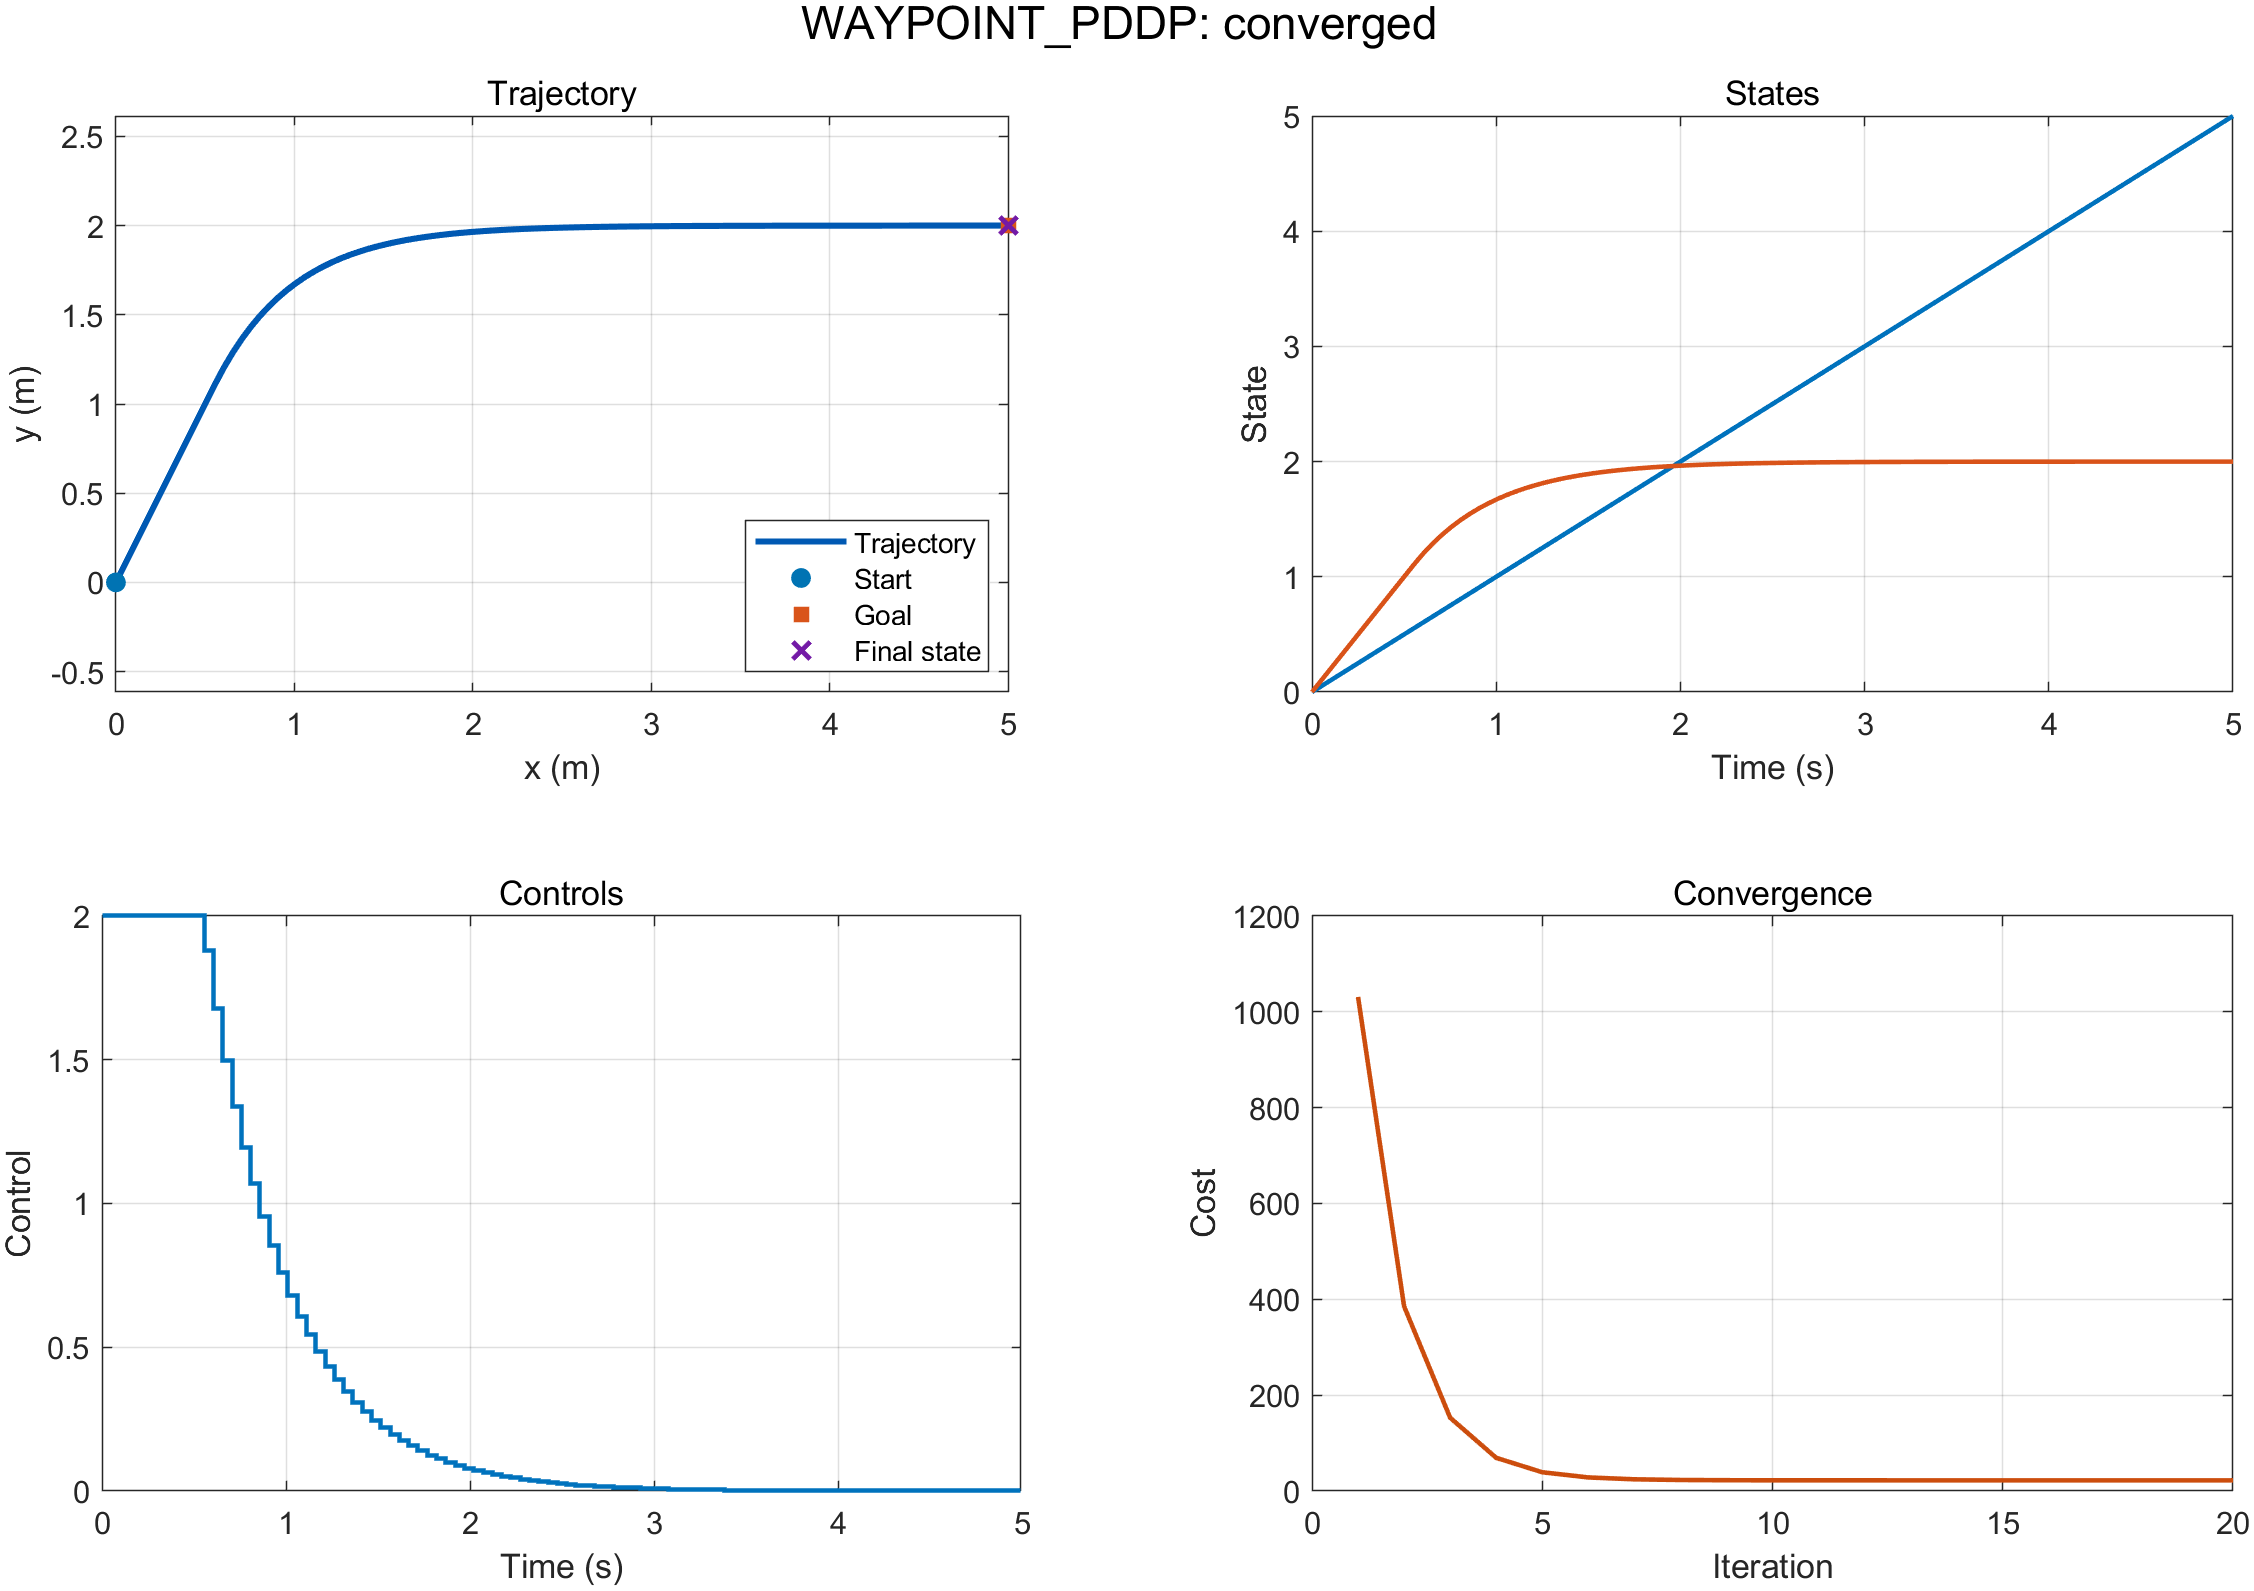
\includegraphics[width=0.96\textwidth]{figures/planar_trajectory.png}
  \caption{二维点质量：轨迹、状态、控制和代价历史}
\end{figure}

\section{终端缺陷曲线机动}

\subsection{优化问题}

状态为 $\bm x=[p_x,p_y,z]^\mathsf{T}$。代码采用
\begin{equation}
  \dot{\bm x}=
  \begin{bmatrix}0\\u\\0\end{bmatrix}+
  \begin{bmatrix}1\\0\\0\end{bmatrix},
  \qquad
  \bm x(0)=
  \begin{bmatrix}0\\0\\0\end{bmatrix},\quad
  \bm x(T)=
  \begin{bmatrix}5\\1.2\\0\end{bmatrix}.
\end{equation}
输入终端时间为 $T=10$，$\Delta t=0.2$，$|u|\le1.5$。目标权重为
\begin{equation}
  Q_f=\diag(200,200,40),\quad
  Q_s=\diag(1,2,0.2),\quad R=0.2.
\end{equation}
\code{terminal_defect_pddp} 以
$\bm d=\bm x_N-\bm x_{\mathrm f}$ 修正反向递推，并使用
$\mathcal M=J+w_d\normtwo{\bm d}$ 评价候选解。测试另在轨迹上设置五个均匀审计边界，检查边界相邻步的 Euler 连续性缺陷；这些边界不是独立射击节点。

\subsection{仿真结果分析}

重新积分后，初始目标为 $2582.98154$，最终目标为 $22.09196962$。

终端误差为
$3.14758\times10^{-7}$，RK4 缺陷为
$1.77636\times10^{-15}$，控制越界为零。轨迹相对起终点直线的最大偏差超过测试要求的 $0.25$，因此算例确实形成曲线机动，而非仅做直线插值。
主迭代接受 29 步，在第 30 轮按代价变化容差停止；返回目标与独立重算一致。初始导引已按实际网格重新积分，不能把新旧初始代价直接比较；代价变化停止也不证明一阶驻点。

\begin{figure}[H]
  \centering
  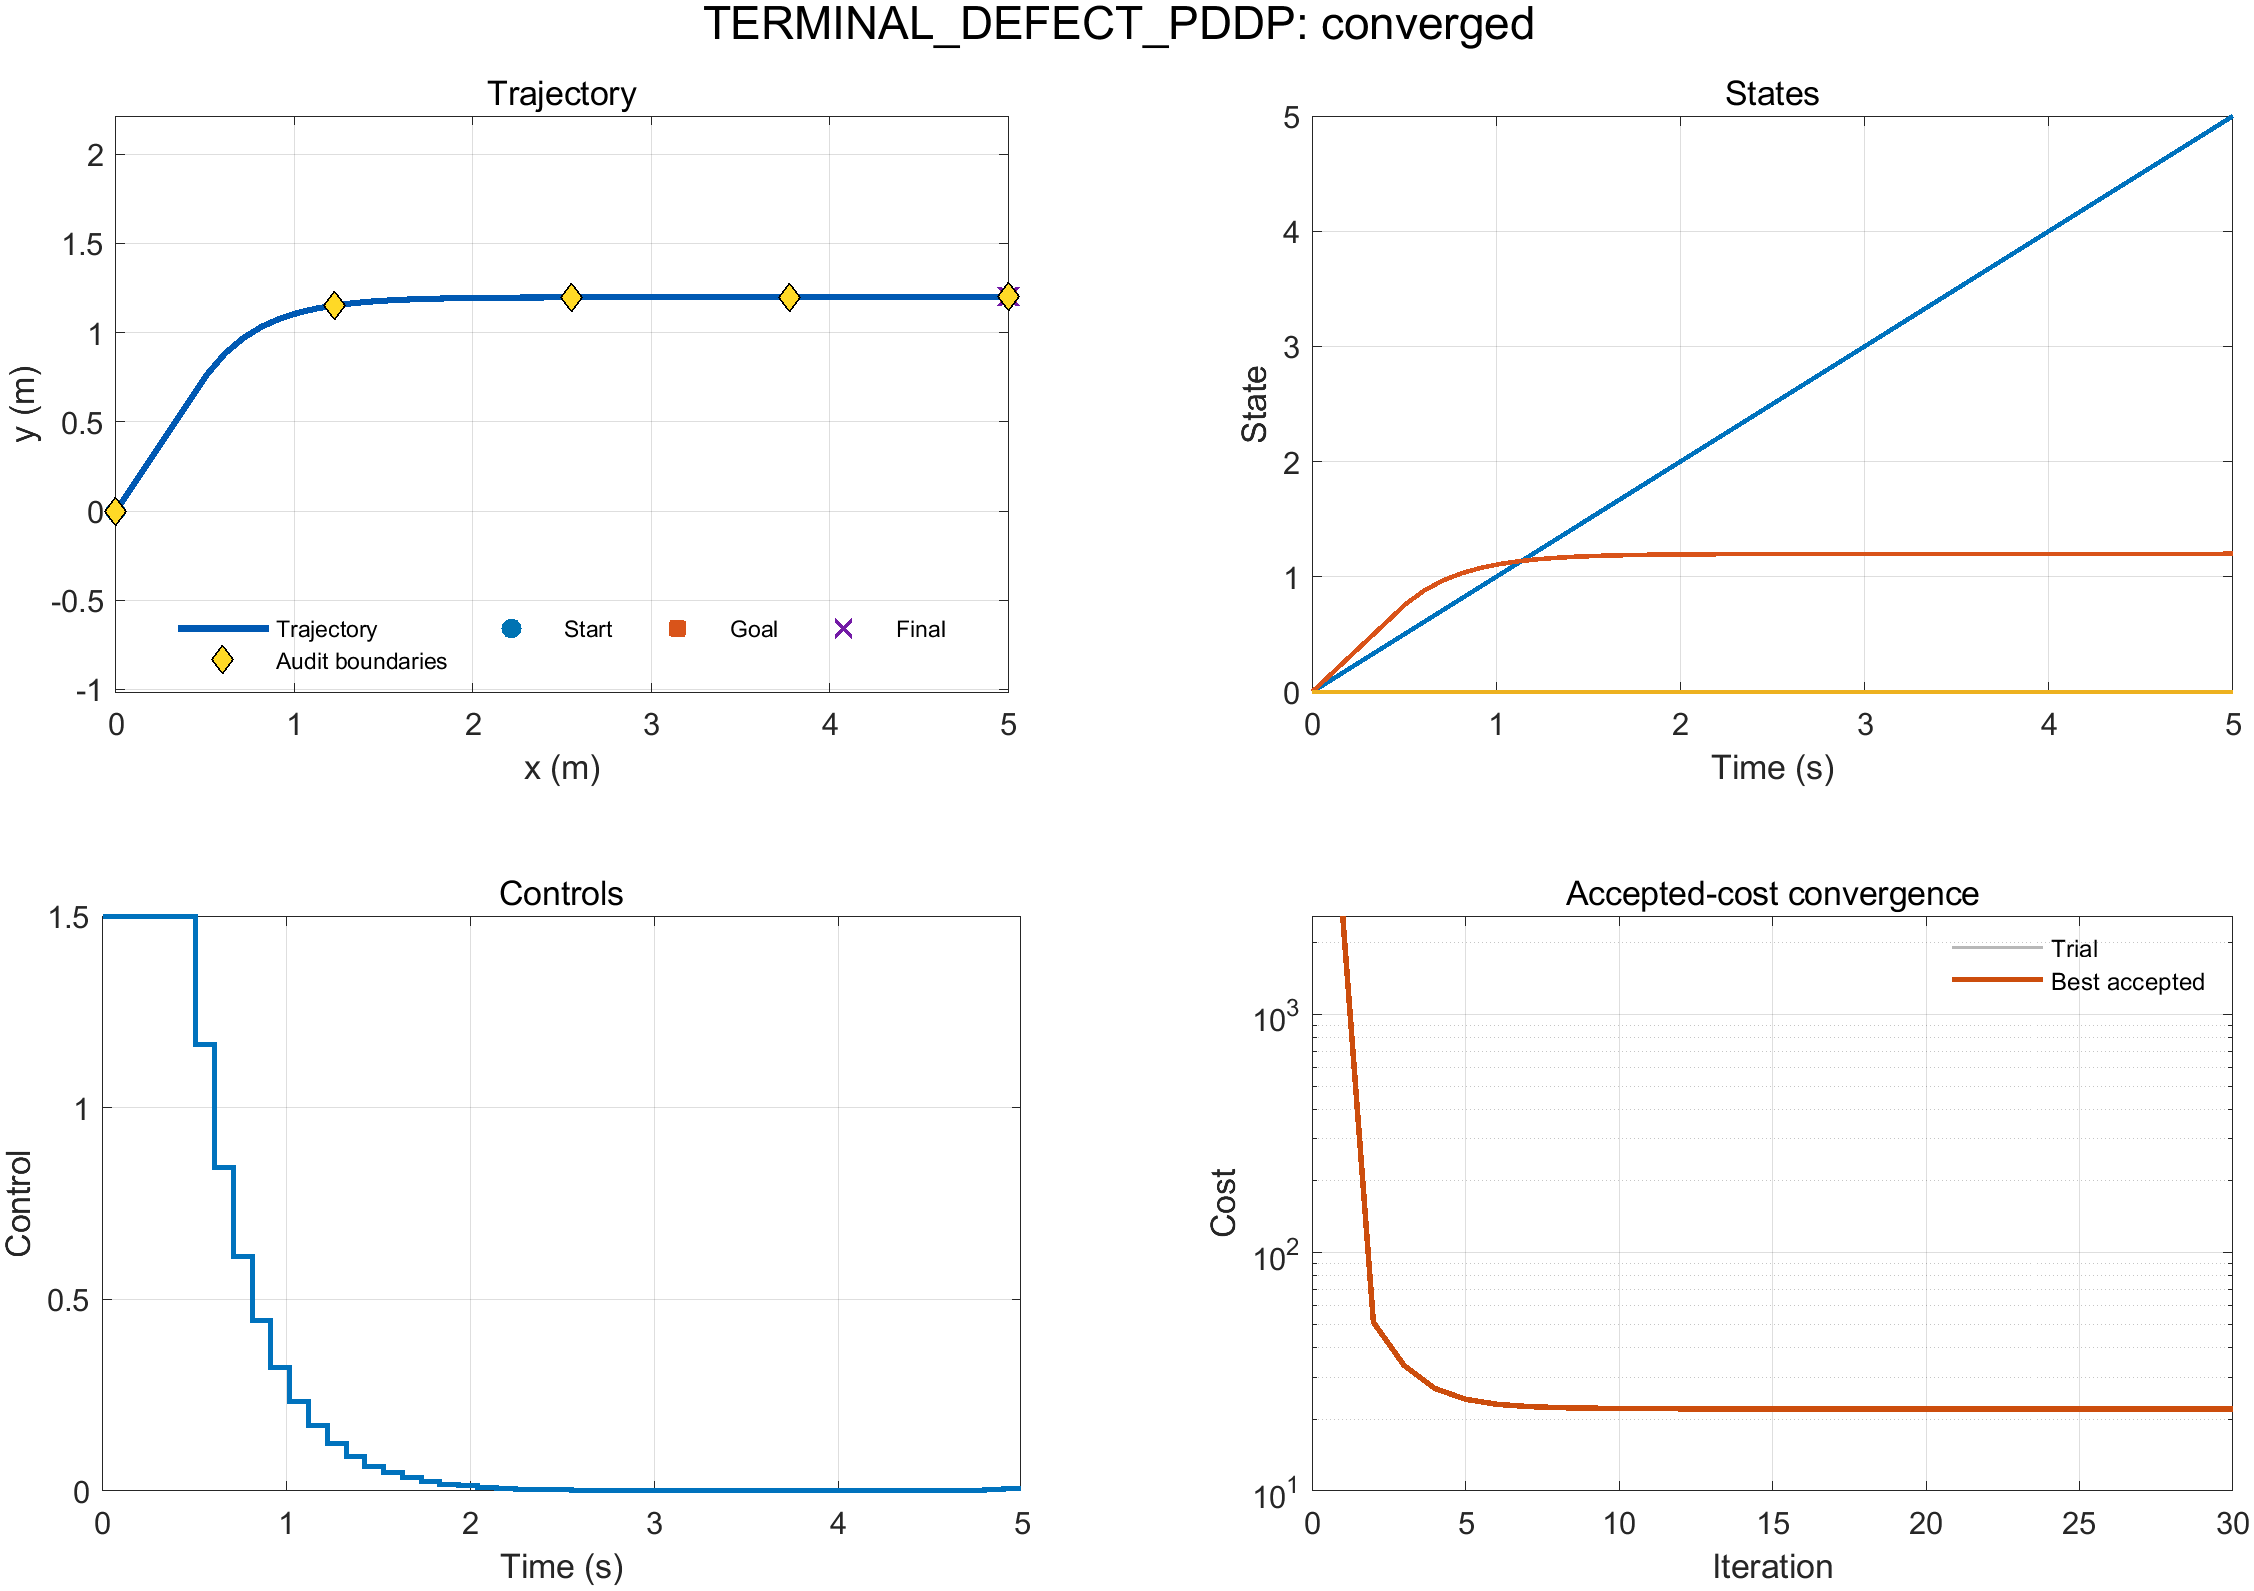
\includegraphics[width=0.96\textwidth]{figures/terminal_defect.png}
  \caption{终端缺陷曲线机动及均匀审计边界}
\end{figure}

\section{二维圆形障碍物规避}

\subsection{优化问题}

状态 $\bm x=[p_x,p_y,\alpha]^\mathsf{T}$ 表示位置和航向角，控制 $u$ 为转向角速度：
\begin{equation}
  \dot p_x=v\cos\alpha,\qquad
  \dot p_y=v\sin\alpha,\qquad
  \dot\alpha=u,\qquad v=1.
\end{equation}
边界、时间和控制约束为
\begin{equation}
  \bm x_0=[0,0,0]^\mathsf{T},\quad
  \bm x_{\mathrm f}=[5,0,0]^\mathsf{T},\quad
  T_0=10,\quad\Delta t_{\mathrm{input}}=0.2,\quad |u|\le1.5,
\end{equation}
并把实际机动时间限制在
\begin{equation}
  5.0\le T\le6.0.
\end{equation}
单个圆形障碍物的中心为 $\bm c=[2.5,0]^\mathsf{T}$，物理半径为
$r=0.22$，安全余量为 $m_{\mathrm{safety}}=0.03$，算法激活余量为
$m_{\mathrm{enforcement}}=0.12$。
几何可行条件为
\begin{equation}
  h(\bm p)=\normtwo{\bm p-\bm c}^2-(r+m_{\mathrm{safety}})^2\ge0.
\end{equation}
障碍物中心位于直线 $p_y=0$ 上，故无障碍直线参考的物理净空为
$-(0.22+0.03)=-0.25<0$，确实穿过障碍物。终端投影阈值和最大迭代数分别为
$5\times10^{-3}$ 和 30。
目标权重为
\begin{equation}
  Q_f=\diag(200,200,40),\quad
  Q_s=\diag(1,1,0.2),\quad R=0.2.
\end{equation}

\subsection{仿真结果分析}

正式示例启用第~\ref{sec:geometry-refinement}~节的多起点控制重启与受界时间优化。原二次目标约为 $J=21.66008$，机动时间为 $5.03221$ s，终端误差 $1.75\times10^{-6}$，精确状态线段净空约 $0.004985$ m，独立局部 RK4 缺陷约 $1.66\times10^{-3}$。全程独立 RK4 的最小净空约 $0.00735$ m，终端误差约 $1.05\times10^{-4}$。

正式图仅展示当前单侧绕行轨迹、实际控制与独立净空验证；两种语言的比较见双语言试验章节。图中轨迹来自真实控制积分，不做输出曲线平滑；这里报告通过指定检查的可行解，不声称全局最优。

\begin{figure}[H]
  \centering
  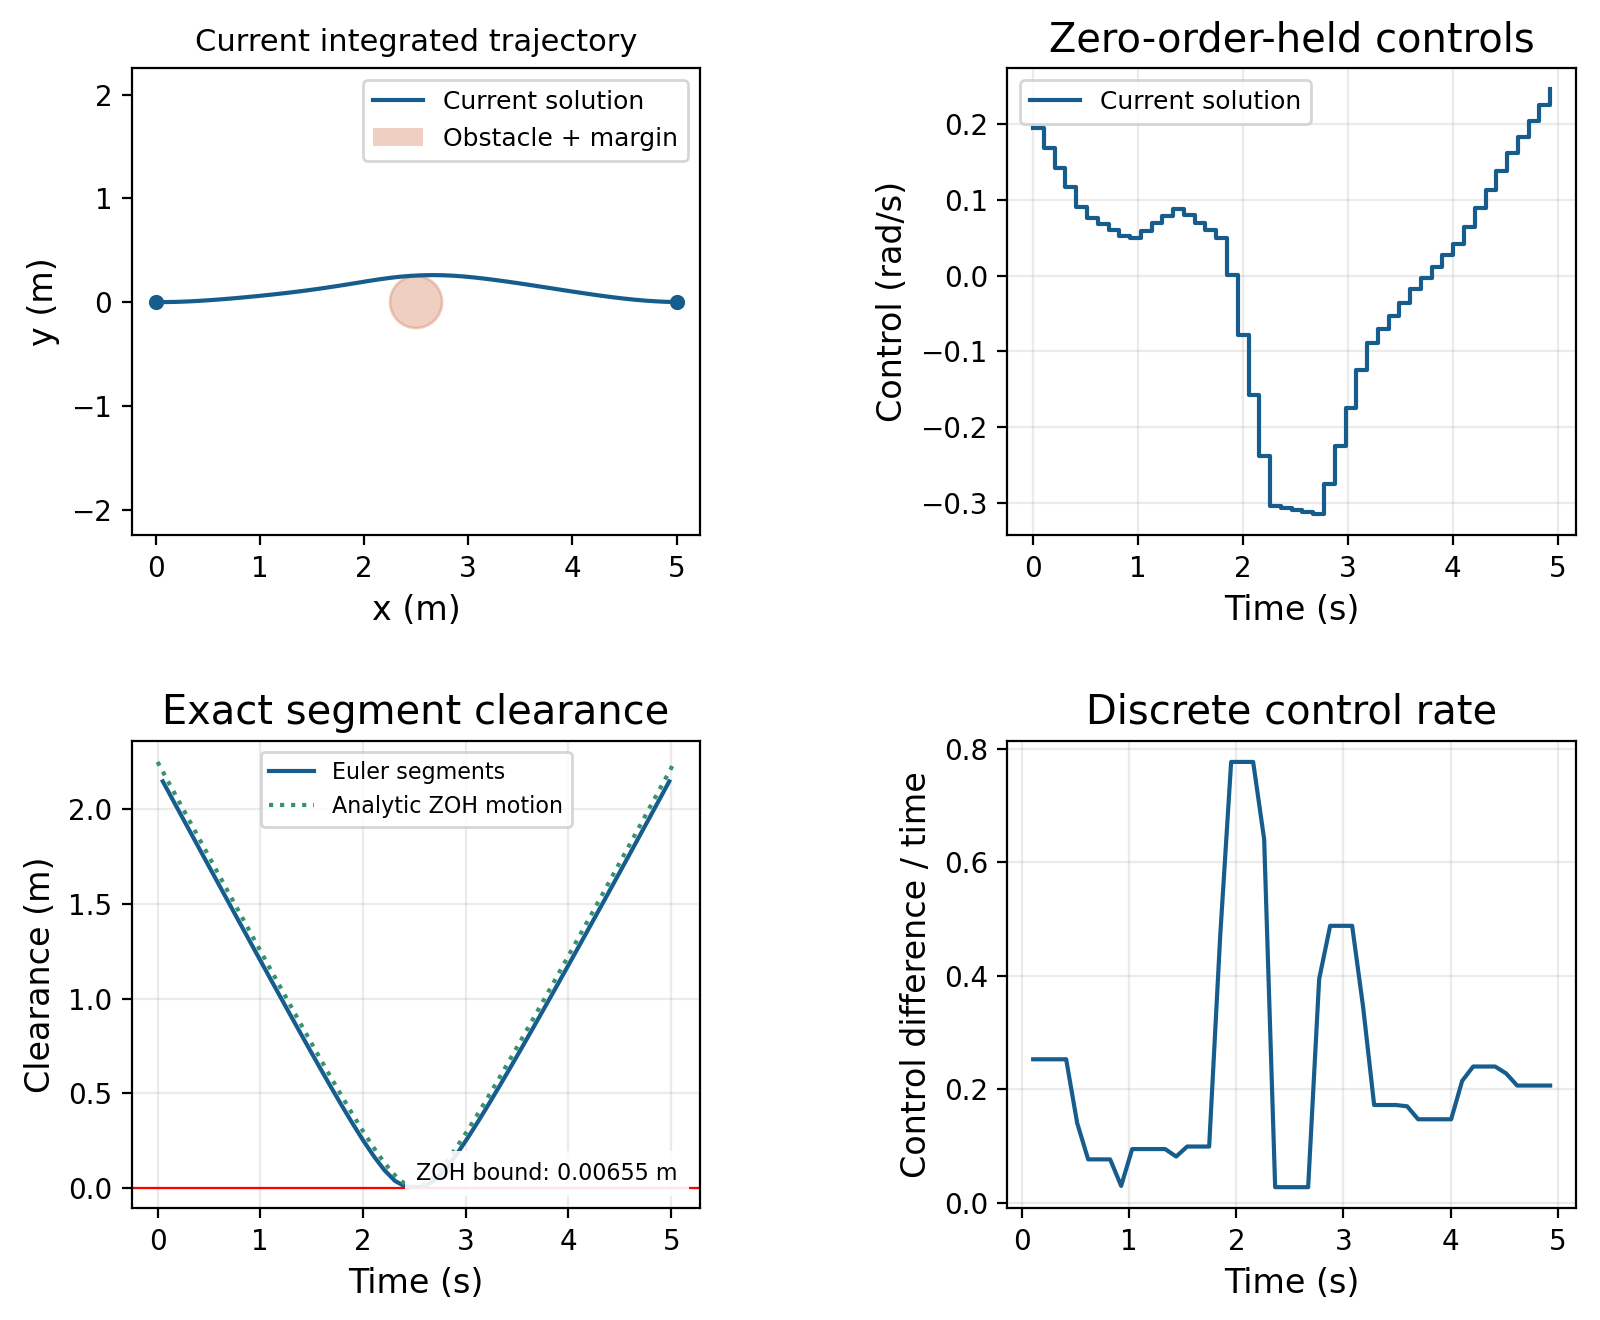
\includegraphics[width=0.96\textwidth]{figures/obstacle_2d.png}
  \caption{二维圆障碍物：当前轨迹、实际控制、独立净空及控制变化}
\end{figure}

\section{三维球形障碍物规避}

\subsection{优化问题}

状态和控制分别为
\begin{equation}
  \bm x=[p_x,p_y,p_z,v,\gamma,\psi]^\mathsf{T},\qquad
  \bm u=[\dot\psi,\dot\gamma]^\mathsf{T}.
\end{equation}
常速三维运动学模型为
\begin{align}
  \dot p_x&=v\cos\gamma\cos\psi,&
  \dot p_y&=v\cos\gamma\sin\psi,\\
  \dot p_z&=v\sin\gamma,&
  \dot v&=0,&
  \dot\gamma&=u_2,&
  \dot\psi&=u_1.
\end{align}
目标位置 $\bm p_{\mathrm f}=[5,2,1]^\mathsf{T}$，并令
\begin{equation}
  v=\frac{\normtwo{\bm p_{\mathrm f}}}{5},\quad
  \gamma=\operatorname{atan2}(1,\sqrt{5^2+2^2}),\quad
  \psi=\operatorname{atan2}(2,5).
\end{equation}
初、末状态使用相同的 $v,\gamma,\psi$，名义时间 $T_0=5$，输入步长
$\Delta t=0.1$，实际机动时间满足 $5.0\le T\le6.0$，且
$|u_1|,|u_2|\le1.5$。目标权重为
\begin{equation}
  Q_f=\diag(1000,1000,1000,20,100,100),
\end{equation}
\begin{equation}
  Q_s=\diag(0.05,0.05,0.05,0.01,0.05,0.05),
  \qquad R=0.2I_2.
\end{equation}
球心为
$\bm c=\frac{24}{49}[5,2,1]^\mathsf{T}
=[2.44898,0.979592,0.489796]^\mathsf{T}$，物理半径 $0.18$，安全余量
$0.04$，算法激活余量为 $0.15$。球心位于起终点线段上，故直线参考物理净空为 $-0.22$。终端投影阈值为 $5\times10^{-3}$。

\subsection{仿真结果分析}

当前返回解的原二次目标为 $J=1.30494$。机动时间为 $5.02108$ s，终端误差 $7.88\times10^{-6}$，精确线段净空约 $0.004997$ m，独立局部 RK4 缺陷约 $9.81\times10^{-4}$。从初始状态全程独立 RK4 积分的最小净空约 $0.00366$ m，终端误差约 $5.97\times10^{-5}$。

当前控制变化能量约为 0.145，轨迹采用平缓的单侧绕行。三维图的第四面板使用起终连线方向的轴向坐标与到该轴的径向距离，避免相机视角遮挡真实绕行偏离；它是对实际积分节点的坐标变换，不改变轨迹。新的窄幅绕行确实更接近障碍物，因此同时展示控制、净空及独立积分检查，不能仅凭图形判断安全。结果是有限维参数化下经过指定检查的局部改善解，不声称全局最优或任意初值收敛。

\begin{figure}[H]
  \centering
  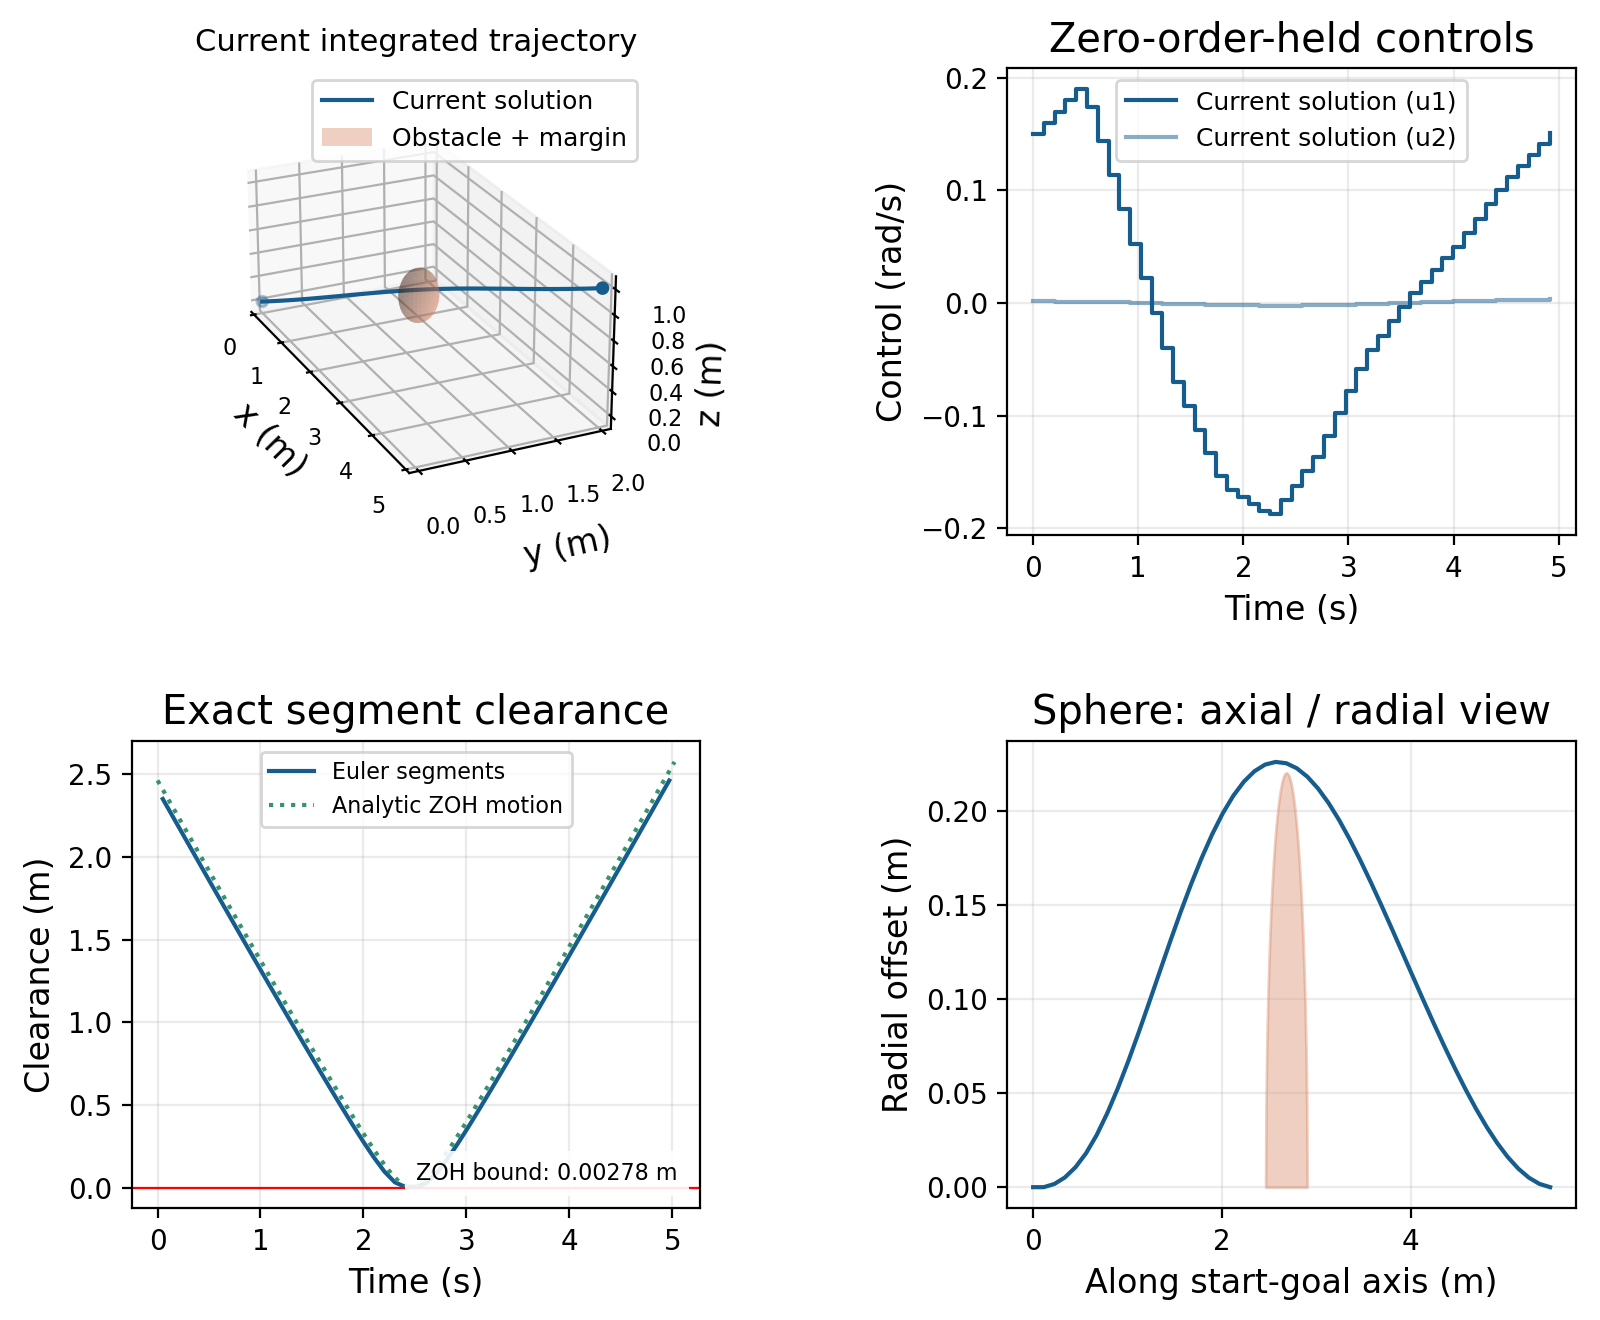
\includegraphics[width=0.96\textwidth]{figures/obstacle_3d.png}
  \caption{三维球障碍物：当前轨迹、实际控制、独立净空及轴向/径向视图}
\end{figure}

\section{反应器浓度误差调节}

\subsection{优化问题}

状态 $x$ 是归一化浓度误差，控制 $u$ 是调节指令。线性模型为
\begin{equation}
  \dot x=-0.30x+0.02u,\qquad
  x(0)=4,\quad x_{\mathrm f}=0,\quad
  T=15,\quad\Delta t=0.3,\quad |u|\le1.
\end{equation}
\code{QuadraticCost\_fft} 实现的目标为
\begin{equation}
  J=100x_N^2+
  \sum_{k=0}^{N-2}\left(x_k^2+u_k^2\right)\Delta t,
\end{equation}
即 $Q_f=200,Q_s=2,R=2$。求解器使用
\code{penalty_free_time_ddp}，并要求末端附近的 $|x|$ 序列不再增长、已接受目标严格递减。

\subsection{仿真结果分析}

目标由 $43.04928$ 降至 $43.02433$，下降 $0.05797\%$；虽然相对改善不大，但终端误差达到
$0.0313922<0.04$。算法接受 3 个迭代、拒绝 10 个候选，停止原因为 trial cost 变化低于阈值；控制无越界，RK4 缺陷为 $0.0157396$。
该结果说明主要调节作用来自系统本身的稳定衰减，优化控制只提供小幅额外改善，因此不能仅用目标下降百分比评价该例。

\begin{figure}[H]
  \centering
  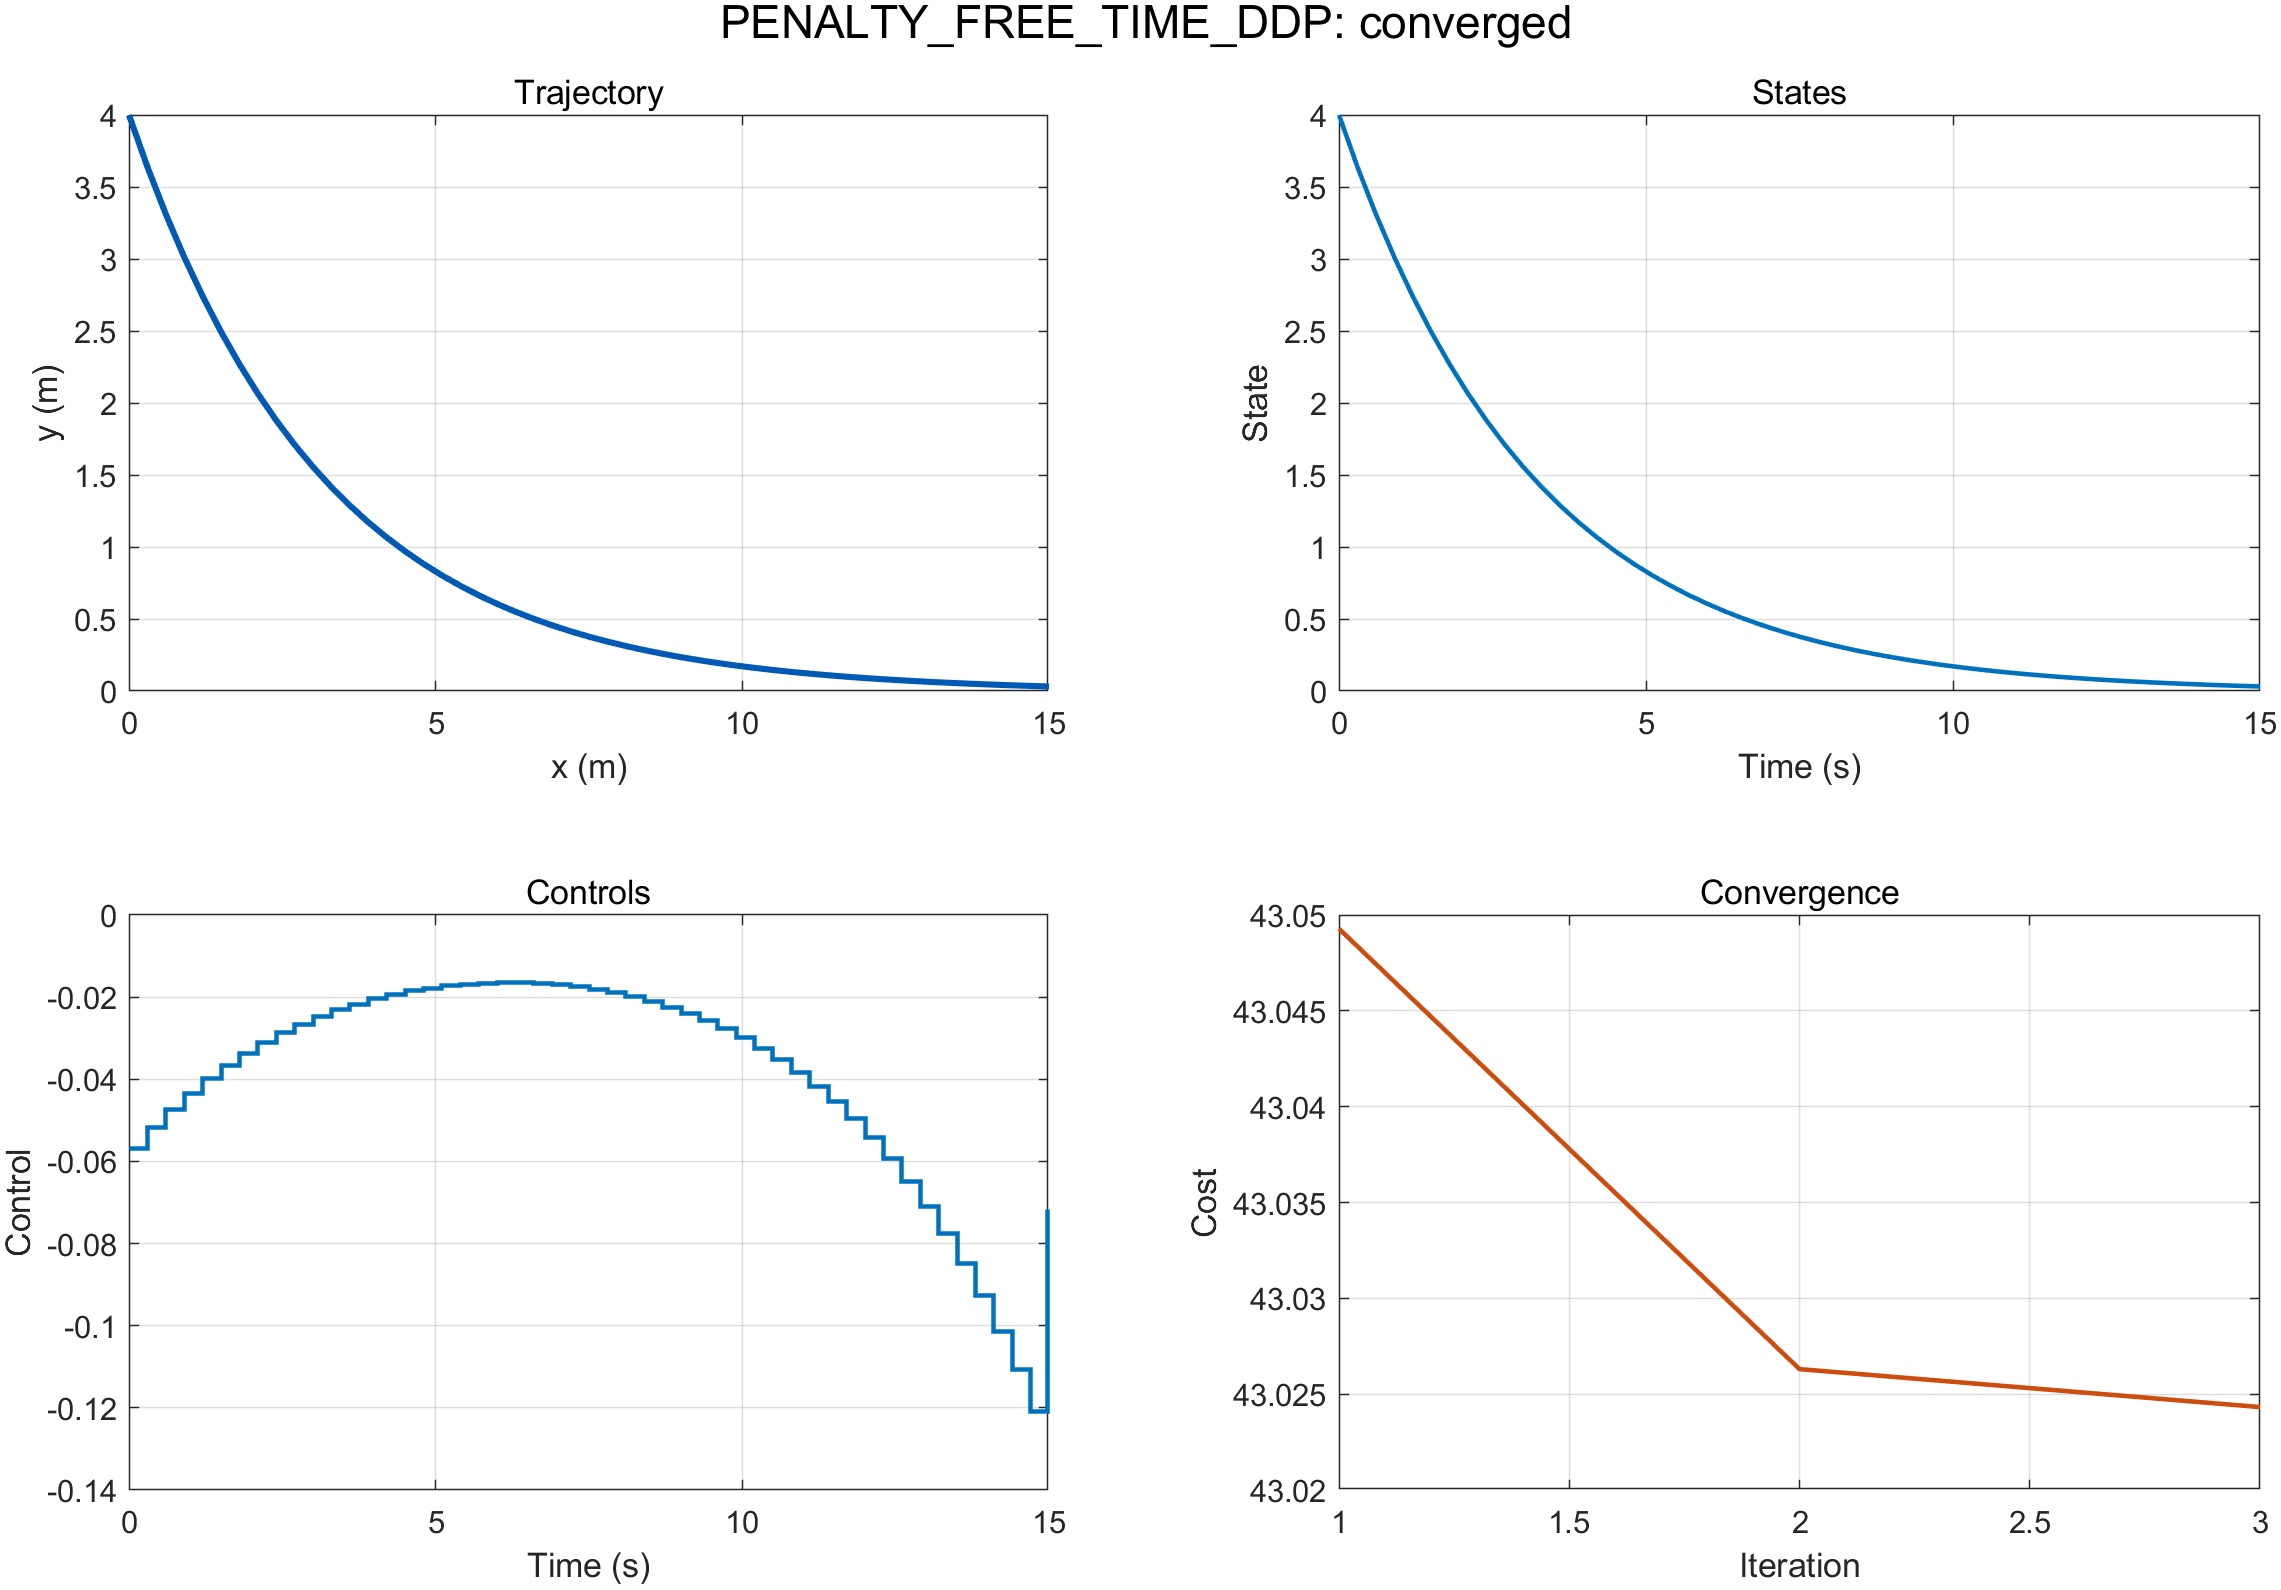
\includegraphics[width=0.96\textwidth]{figures/reactor_regulation.png}
  \caption{反应器浓度误差调节：状态衰减、控制和严格已接受代价}
\end{figure}

\section{柔性安装振动抑制}

\subsection{优化问题}

状态 $\bm x=[q,\dot q]^\mathsf{T}$ 分别为位移和速度，控制 $u$ 为驱动指令：
\begin{equation}
  \dot{\bm x}=
  \begin{bmatrix}
    0&1\\-1&-0.4
  \end{bmatrix}\bm x+
  \begin{bmatrix}0\\0.2\end{bmatrix}u.
\end{equation}
边界、约束和权重为
\begin{equation}
  \bm x_0=[1.2,0]^\mathsf{T},\quad
  \bm x_{\mathrm f}=[0,0]^\mathsf{T},\quad
  T_0=15,\quad\Delta t=0.3,\quad |u|\le2,
\end{equation}
\begin{equation}
  Q_f=\diag(200,60),\quad
  Q_s=\diag(2,0.5),\quad R=0.5.
\end{equation}
\code{free_time_pddp} 同时调整控制序列和标量终端时间。

\subsection{仿真结果分析}

目标由 $22.8159$ 降至 $4.09081$，下降 $82.070\%$；34 次迭代后终端误差为
$0.00218775<0.01$，控制越界为零。状态曲线显示振动幅值逐步衰减，控制在前期提供主要阻尼作用，后期趋近零。
独立 RK4 缺陷为 $0.0591426$，明显大于线性点质量算例，说明较粗的 $\Delta t=0.3$ 对振荡系统造成可见的 Euler/RK4 离散差异；使用结果时应同时报告这一数值误差。

\begin{figure}[H]
  \centering
  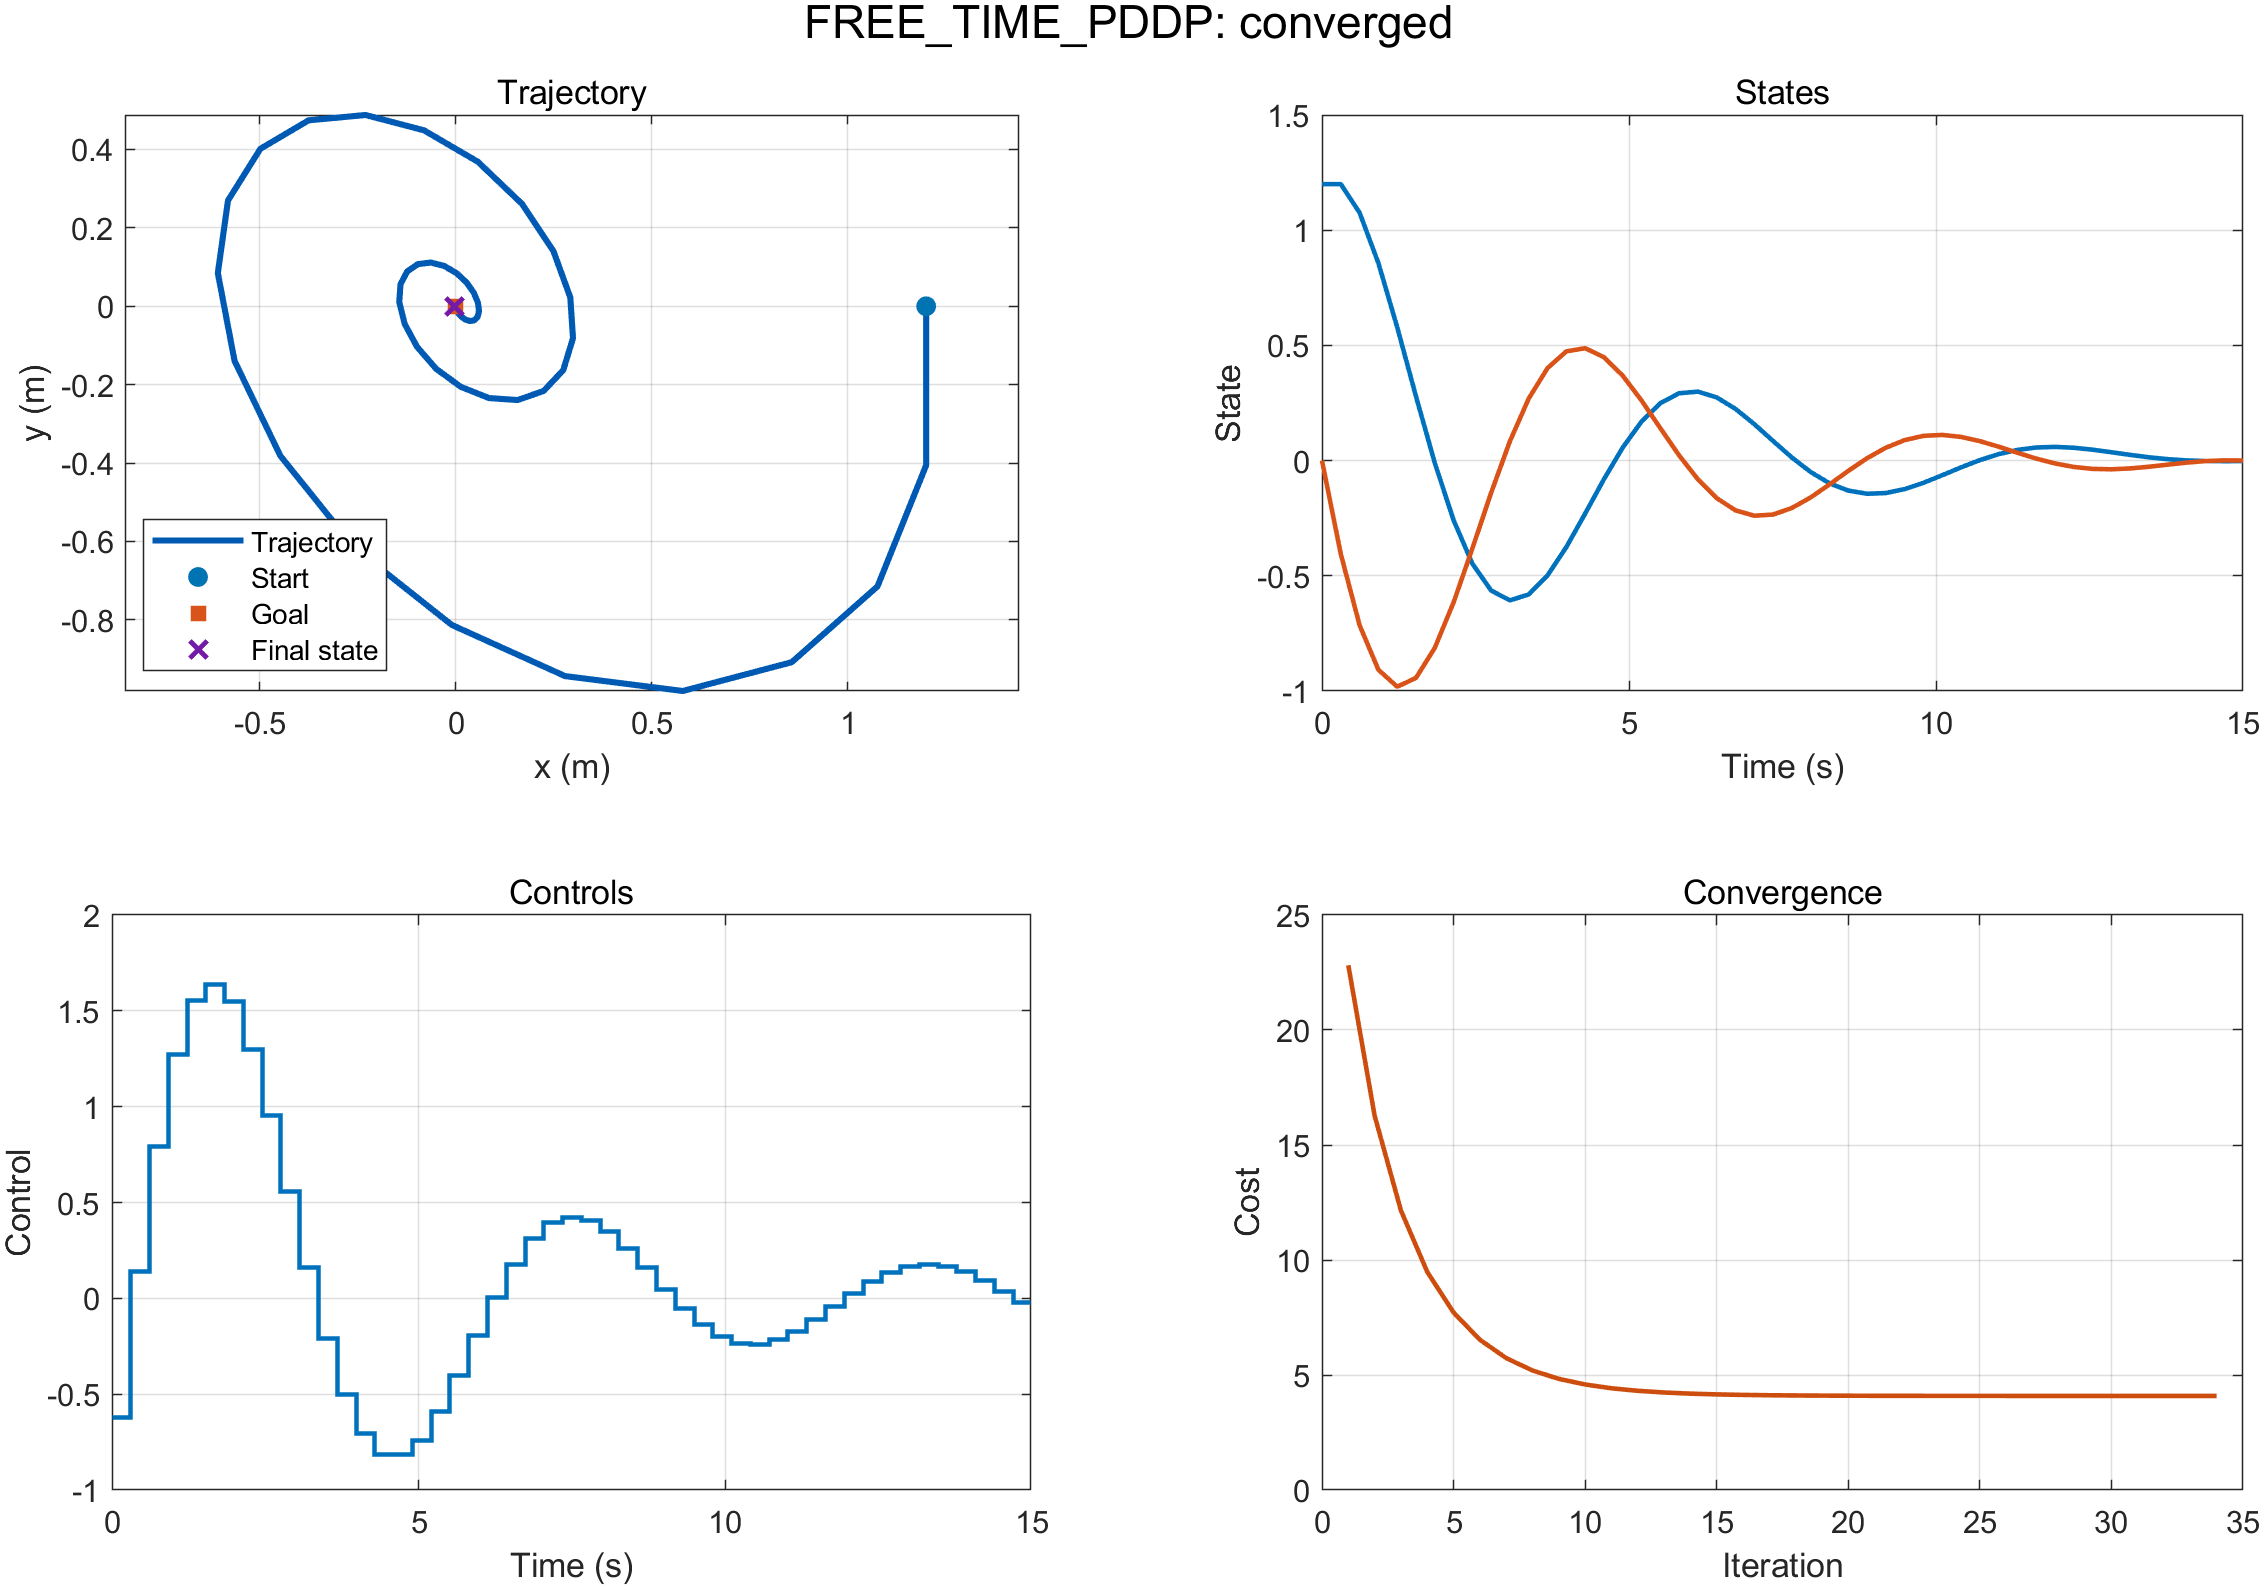
\includegraphics[width=0.96\textwidth]{figures/vibration_regulation.png}
  \caption{柔性安装振动抑制：状态、控制、自由时间与代价变化}
\end{figure}

\section{倒立摆摆起}

\subsection{优化问题}

状态 $\bm x=[\theta,\omega]^\mathsf{T}$，控制 $u$ 为力矩。参数
$m=1\,\mathrm{kg}$、$l=1\,\mathrm m$、$g=9.81\,\mathrm{m/s^2}$、阻尼 $b=0.1$，动力学为
\begin{equation}
  \dot\theta=\omega,\qquad
  \dot\omega=
  \frac{mgl\sin\theta+u-b\omega}{ml^2}.
\end{equation}
边界与约束为
\begin{equation}
  \bm x_0=[\pi,0]^\mathsf{T},\quad
  \bm x_{\mathrm f}=[0,0]^\mathsf{T},\quad
  T=5,\quad\Delta t=0.05,\quad |u|\le10.
\end{equation}
目标权重为
\begin{equation}
  Q_f=\diag(100,10),\quad
  Q_s=\diag(1,0.1),\quad R=0.1.
\end{equation}
角度是周期变量，因此统一指标层使用
\begin{equation}
  e_T=
  \sqrt{
    \operatorname{wrap}_{[-\pi,\pi)}
    (\theta_N-\theta_{\mathrm f})^2+
    (\omega_N-\omega_{\mathrm f})^2
  }.
\end{equation}
该自定义终端误差由 \code{problem.terminal_error_function} 提供；算例不再手工修改
\code{solution.success} 或 \code{solution.status}。

\subsection{仿真结果分析}

目标由 $518.1542$ 降至 $6.38557$，下降 $98.768\%$。周期角度终端误差为
$2.14796\times10^{-6}$，远低于 $0.01$；控制越界为零。82 次迭代形成先注入能量、再制动捕获直立平衡的控制序列。
RK4 缺陷为 $0.0337196$，反映强非线性摆起过程中 Euler 离散与高精度积分的差异。

\begin{figure}[H]
  \centering
  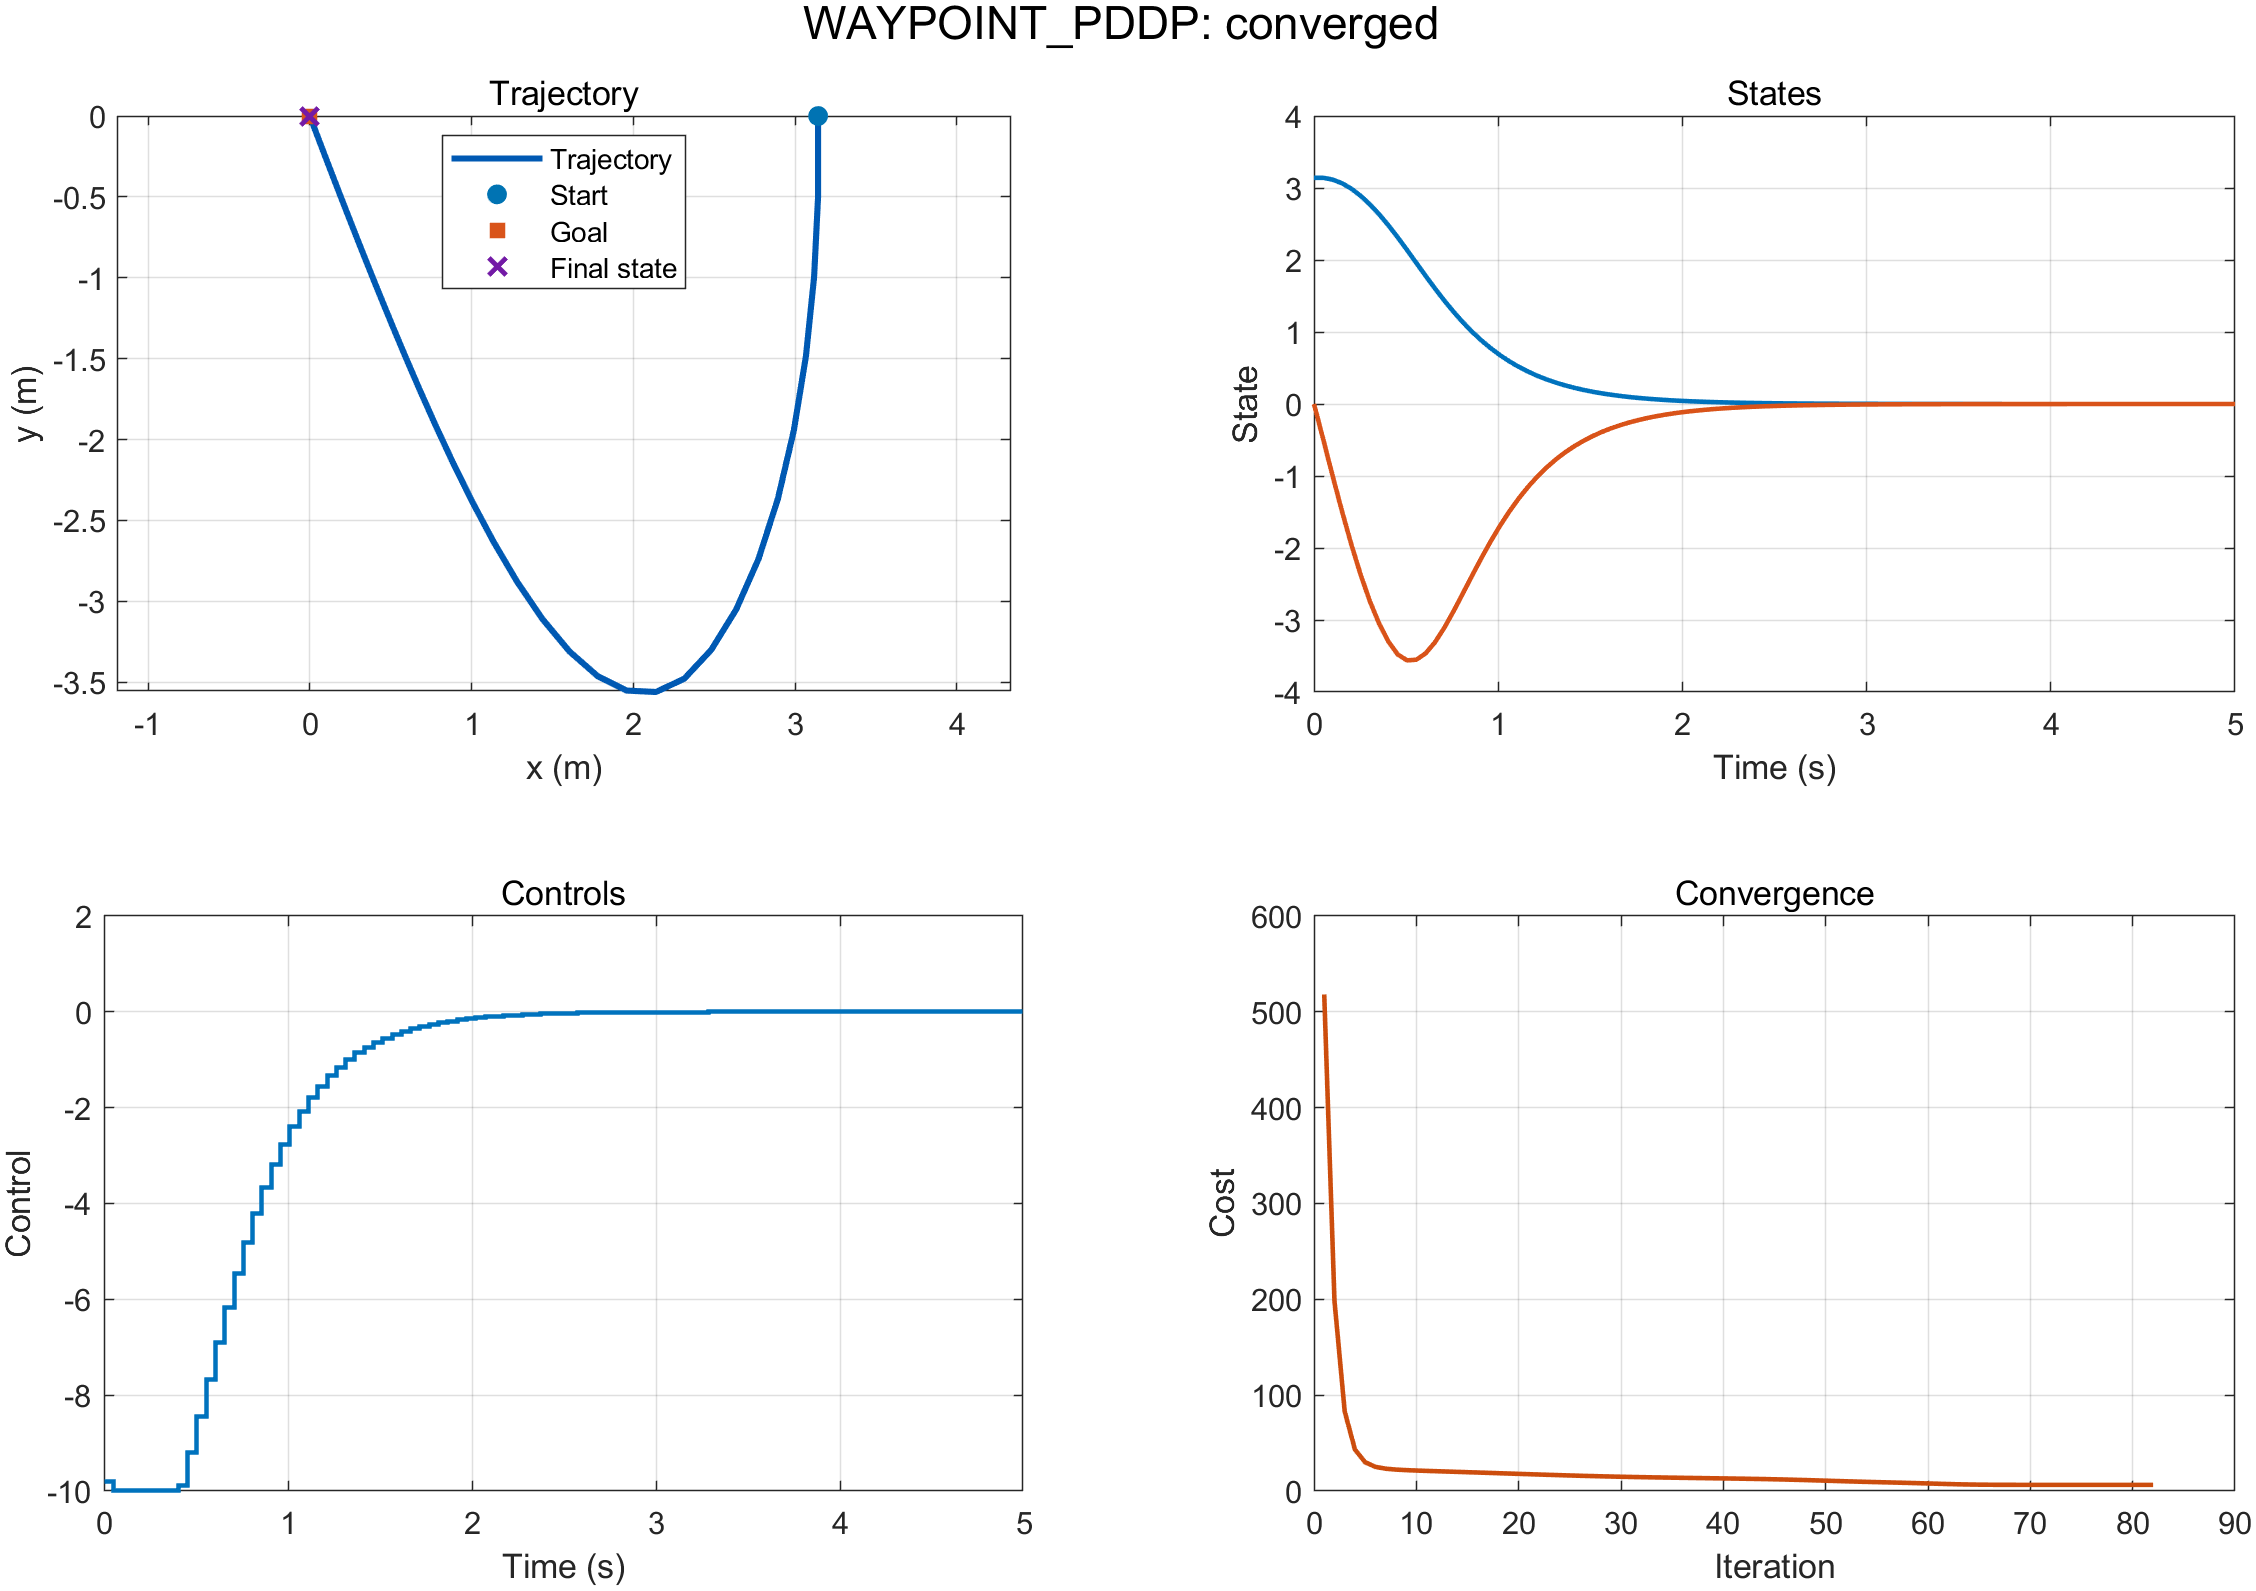
\includegraphics[width=0.96\textwidth]{figures/pendulum.png}
  \caption{倒立摆摆起：周期角度状态、力矩与目标历史}
\end{figure}

\section{非线性热过程调节}

\subsection{优化问题}

状态 $x$ 为归一化温度偏差，$u$ 为带符号的加热/冷却指令：
\begin{equation}
  \dot{x}=-0.25x-0.03x^3+0.60u,
\end{equation}
\begin{equation}
  x_0=2,\quad x_{\mathrm f}=0.032535,\quad
  T=15,\quad\Delta t=0.3,\quad |u|\le1.5.
\end{equation}
目标权重 $Q_f=120,Q_s=2.5,R=0.25$，即
\begin{equation}
  J=60(x_N-0.032535)^2+
  \sum_{k=0}^{N-2}
  \left(1.25(x_k-0.032535)^2+0.125u_k^2\right)\Delta t.
\end{equation}
三次项表示温差较大时增强的被动散热；控制正负分别表示加热和冷却。该例定义 15 秒无执行器输入的被动冷却计划。对 $u_k=0$，离散模型为
\begin{equation}
  x_{k+1}=x_k+0.3\left(-0.25x_k-0.03x_k^3\right),
  \qquad k=0,\ldots,49,
\end{equation}
由 $x_0=2$ 递推得到 $x_{50}=0.0325349083$，公开目标
$0.032535$ 是该模型预测值保留六位小数后的结果。

\subsection{仿真结果分析}

初始和返回目标均为 $22.88081$，严格历史最优解为零执行器输入；终端误差为
$9.17\times10^{-8}<5\times10^{-5}$，控制越界为零，RK4 缺陷为 $0.0184046$。
温度偏差按非线性散热规律平滑衰减并在图形分辨率下与目标重合。试探代价变化在第 198 次达到停止阈值，返回严格历史最优轨迹，并报告 \code{converged_by_cost_change}。这说明求解流程达到其实现的代价变化判据，但仍不等同于一阶驻点证明。

\begin{figure}[H]
  \centering
  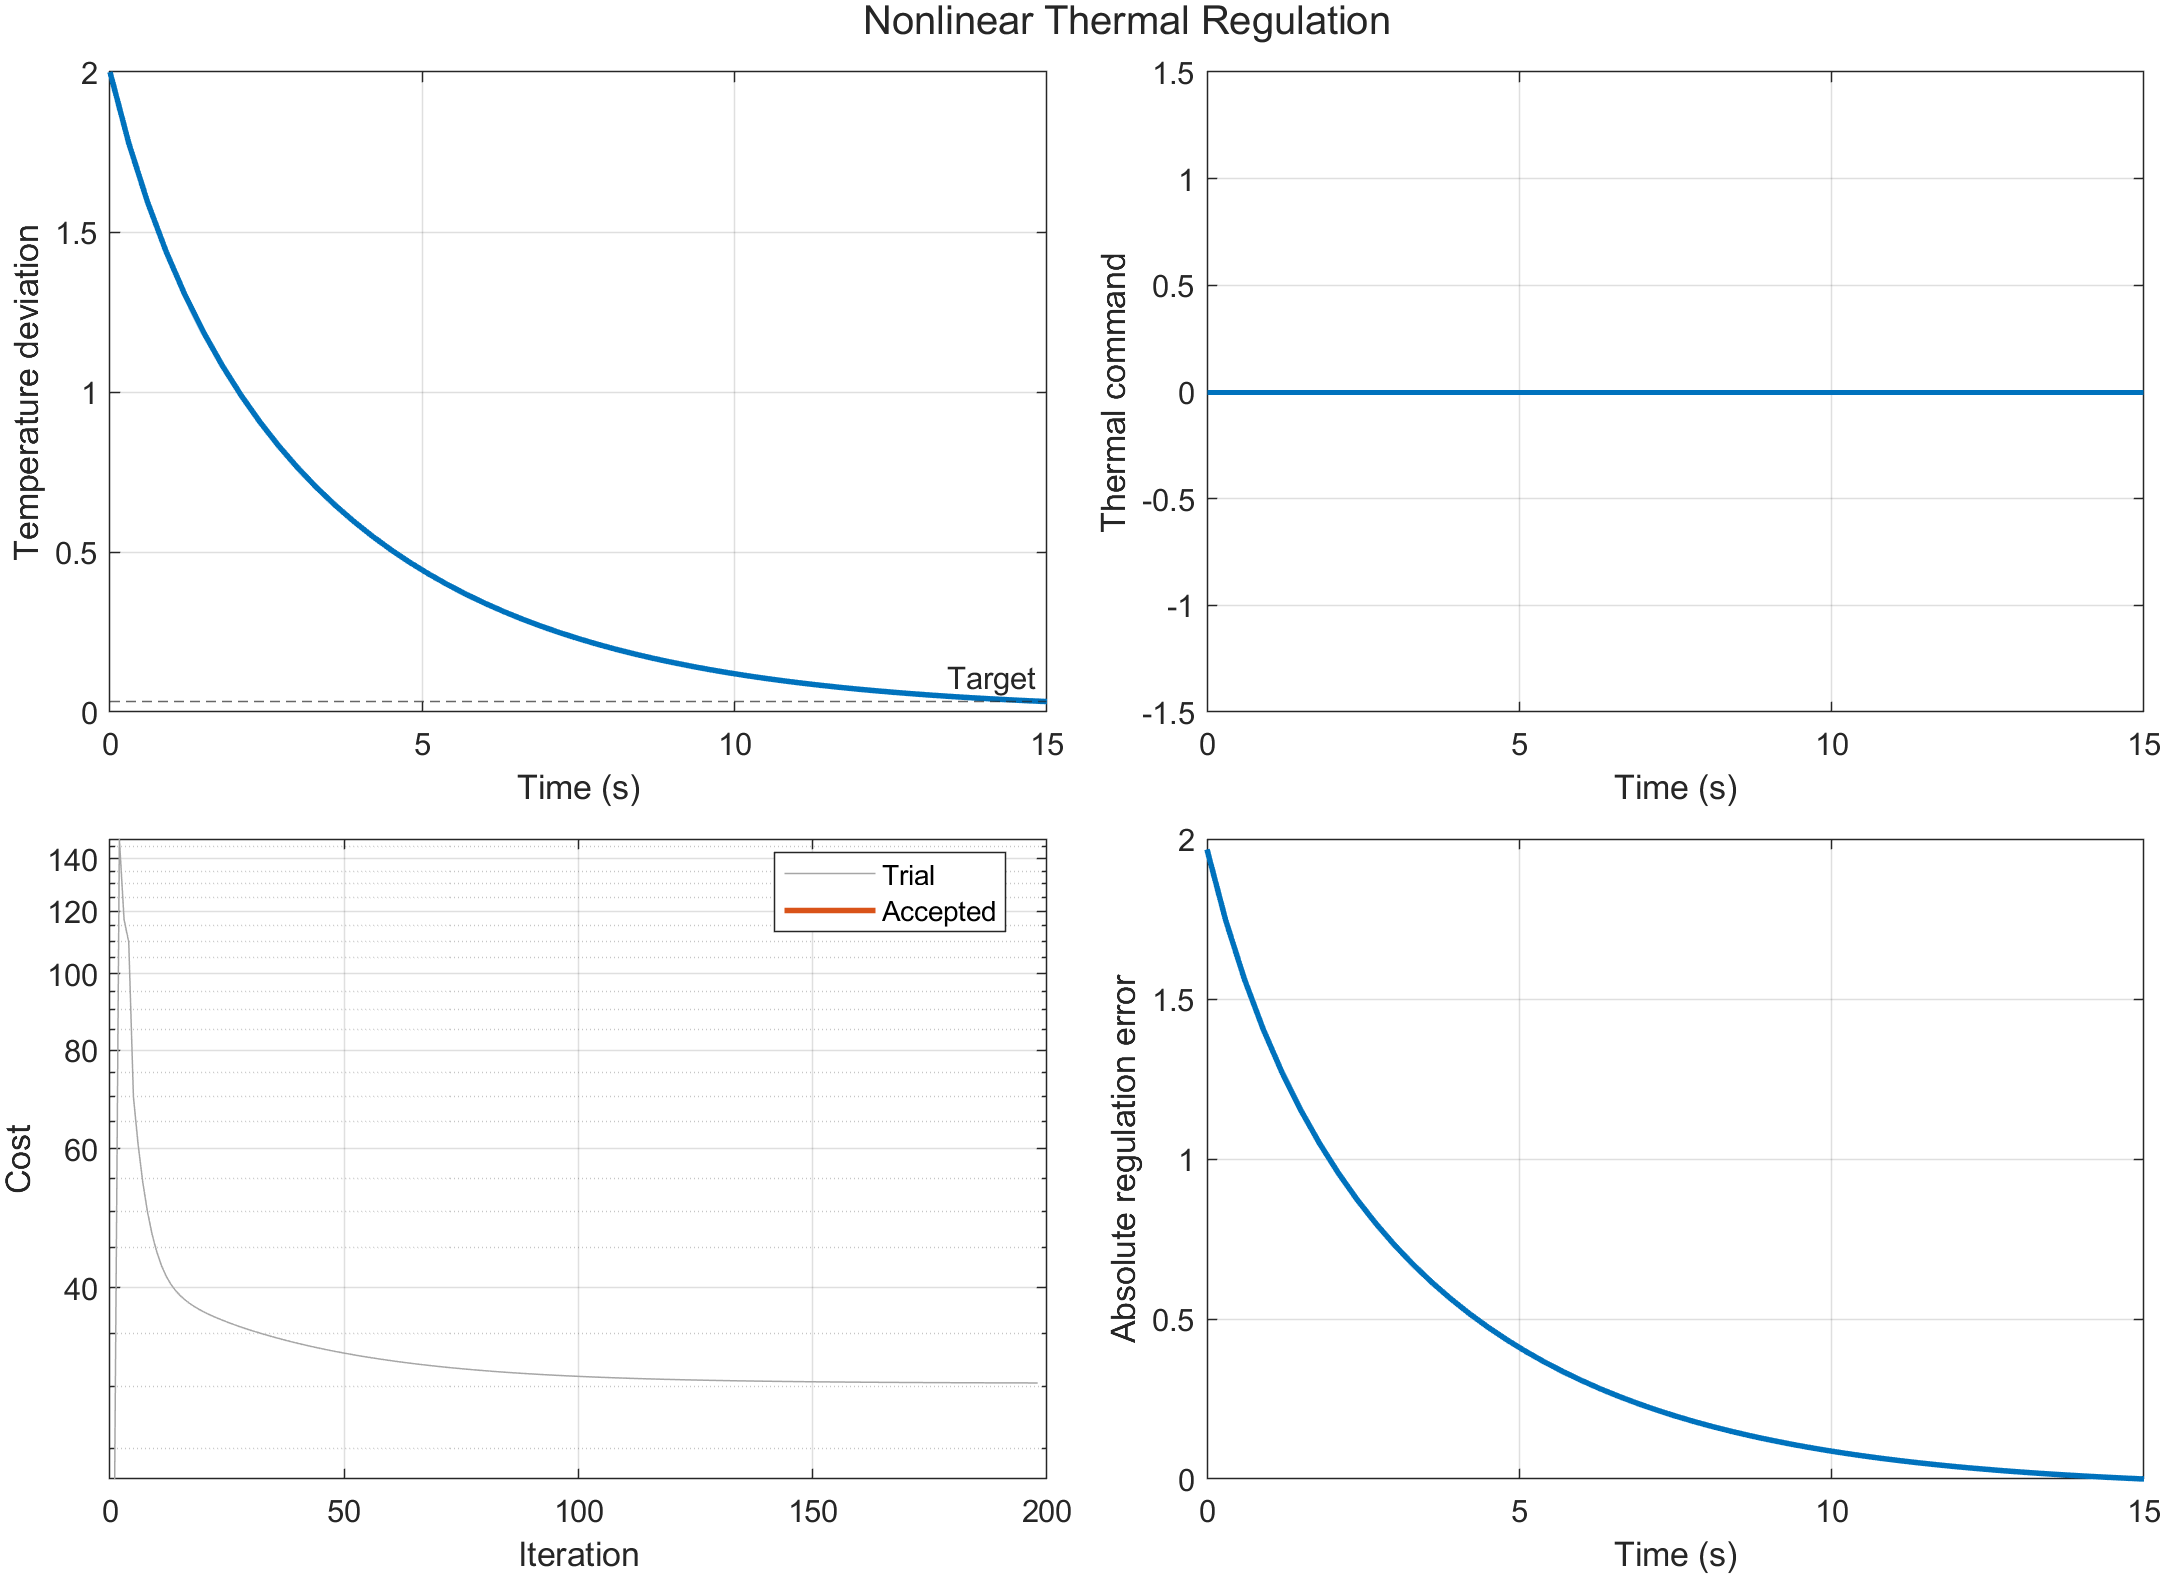
\includegraphics[width=0.96\textwidth]{figures/thermal_regulation.png}
  \caption{非线性热调节：温差、热指令、目标历史和绝对误差}
\end{figure}

\section{带下界的储能管理}

\subsection{优化问题}

状态 $x$ 为归一化储能水平，$u$ 为带符号充放电指令：
\begin{equation}
  \dot{x}=-0.03x+0.08u-0.005.
\end{equation}
参数和约束为
\begin{equation}
  x_0=0.65,\quad x_{\mathrm f}=0.353,\quad
  T=15,\quad\Delta t=0.3,\quad
  |u|\le0.8,\quad x\ge0.25.
\end{equation}
状态下界采用 DDPACK 的正可行约定
\begin{equation}
  G(x)=x-0.25\ge0.
\end{equation}
目标权重 $Q_f=160,Q_s=3,R=0.30$，即
\begin{equation}
  J=80(x_N-0.353)^2+
  \sum_{k=0}^{N-2}
  \left[
    1.5(x_k-0.353)^2+0.15u_k^2
  \right]\Delta t.
\end{equation}
该例定义的是无外部充放电时的被动放电储备计划。对 $u_k=0$，Euler 离散模型为
\begin{equation}
  x_{k+1}=0.991x_k-0.0015,\qquad k=0,\ldots,49,
\end{equation}
因此解析递推给出 $x_{50}=0.3530032229$；公开目标 $0.353$ 是这一计划值保留三位小数后的结果。

\subsection{仿真结果分析}

终端状态为 $0.3530032229$，终端误差仅
$3.22292\times10^{-6}<5\times10^{-5}$；状态下界和控制上界违反量均为零，RK4 缺陷为
$3.29760\times10^{-5}$。归档目标为 $15.60931$，零控制初始轨迹是唯一严格接受的轨迹，随后 85 个候选被拒绝，并以
\code{trial_cost_change_below_tolerance} 停止。
因此，本例验证的是“被动放电按计划抵达储备水平并始终满足下界”，不是主动充放电经济调度基准；零控制是场景定义的一部分，不能被描述为算法发现了复杂的充放电策略。

\begin{figure}[H]
  \centering
  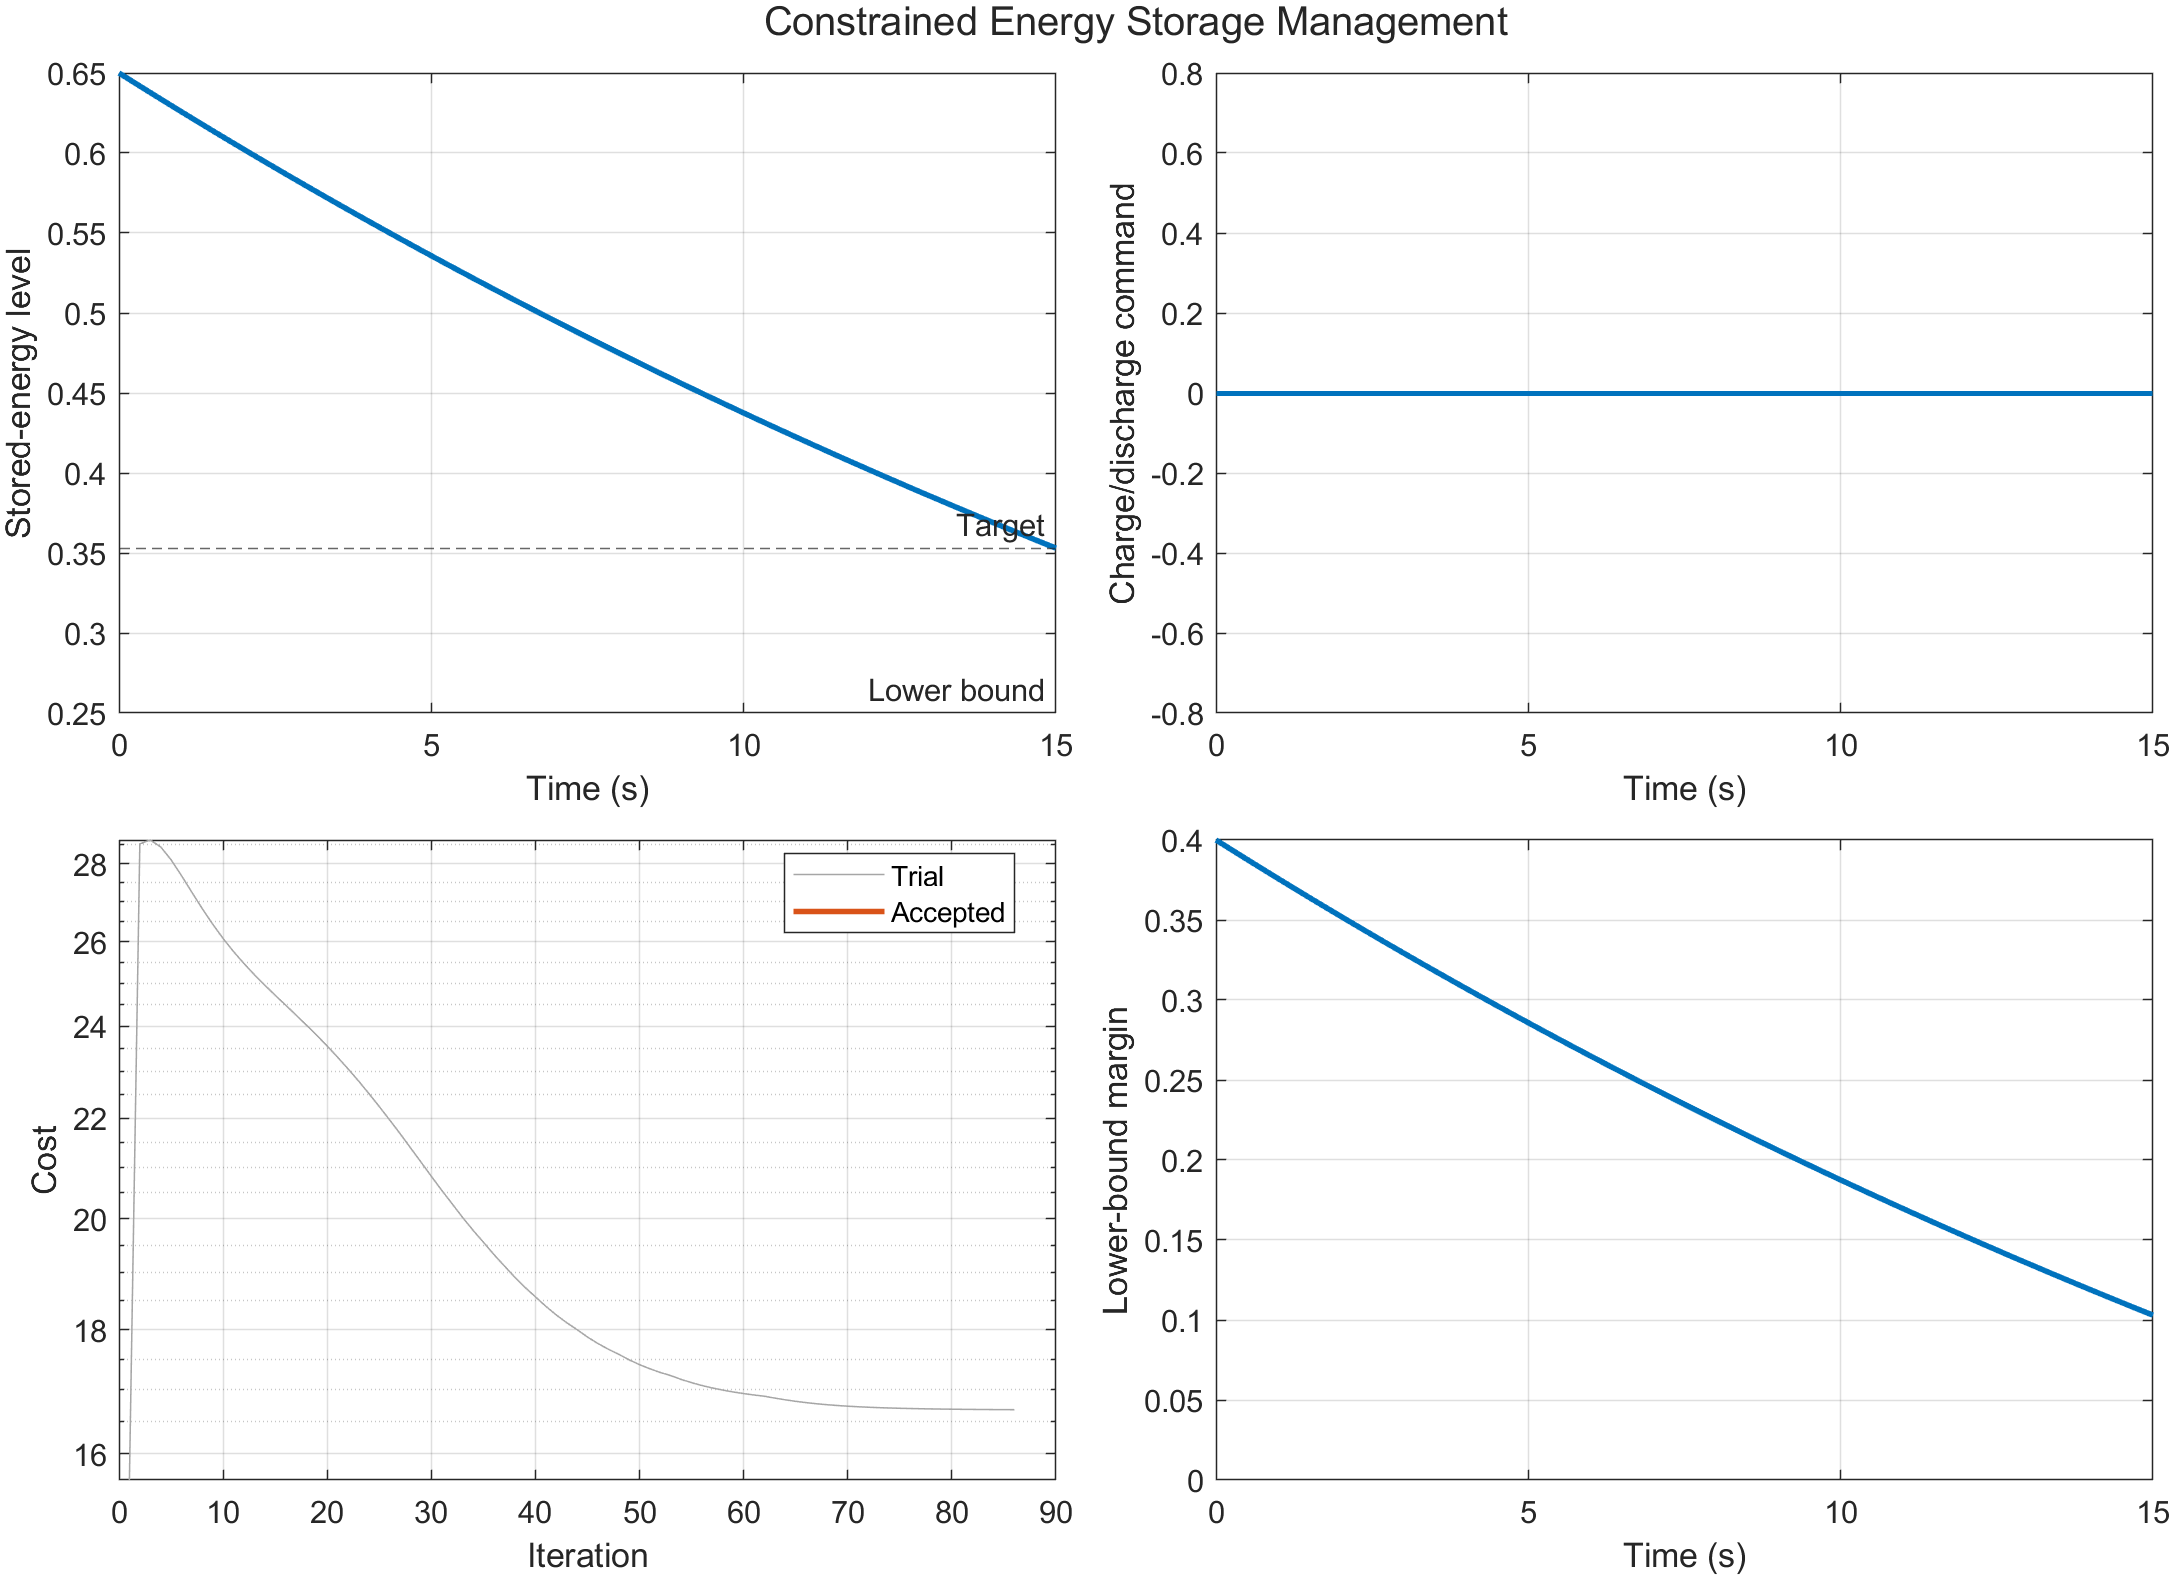
\includegraphics[width=0.96\textwidth]{figures/energy_storage.png}
  \caption{储能管理：储能水平、控制、目标历史和下界余量}
\end{figure}

\section{正式示例数值汇总}

下表来自固定随机种子的正式运行，原始结果位于
运行 \code{run_publication_examples} 指定的输出目录。
运行时间依赖机器与 MATLAB 状态；“迭代”列为记录的实际迭代数。

{\small
\begin{longtable}{p{0.22\textwidth}rrrrr}
\toprule
示例 & $J_0$ & $J_f$ & $\eta_J$ & $e_T$ & 迭代\\
\midrule
\endhead
二维点质量 & 1031.15 & 22.2084 & 97.85\% & $1.22{\times}10^{-4}$ & 20\\
终端缺陷轨迹 & 2582.98 & 22.0920 & 99.14\% & $3.15{\times}10^{-7}$ & 30\\
二维几何安全 & 121.742 & 21.6601 & 82.21\% & $1.75{\times}10^{-6}$ & 8+重启\\
三维几何安全 & 6601.43 & 1.30494 & 99.98\% & $7.88{\times}10^{-6}$ & 6+重启\\
反应器调节 & 43.0493 & 43.0243 & 0.058\% & $3.14{\times}10^{-2}$ & 13\\
振动调节 & 22.8159 & 4.09081 & 82.07\% & $2.19{\times}10^{-3}$ & 34\\
倒立摆 & 518.154 & 6.38557 & 98.77\% & $2.15{\times}10^{-6}$ & 82\\
热调节 & 22.8808 & 22.8808 & 0\% & $9.17{\times}10^{-8}$ & 198\\
储能管理 & 15.6093 & 15.6093 & 0\% & $3.22{\times}10^{-6}$ & 86\\
\bottomrule
\end{longtable}
}

\chapter{C++ 使用与双语言对比试验}
\label{chap:dual-language}

\section{语言分工与安装}

完整 MATLAB 包位于 \code{matlab/}，包含原有求解器、模型、公共接口、图形、MAT 文件保存与读取、全部正式和历史示例。原生 C++17 包位于 \code{cpp/}，不依赖 MATLAB、MATLAB Runtime 或 MEX；顶层 \code{CMakeLists.txt} 只构建 C++。本说明书、论文草稿、投稿元数据和 \code{experiments/} 为两种语言共享。MATLAB 从仓库根目录执行 \code{addpath('matlab/tools')} 后调用 \code{setup_ddpack}；外部旧脚本中的安装路径需要相应更新。

C++ 需要 CMake 3.20 以上、C++17 编译器与 Eigen 3.4 以上。先在系统中安装 Eigen，或者配置时用 \code{-DDDPACK_EIGEN_DIR=/path/to/eigen} 指定其源码目录。Linux/macOS 的典型命令如下；Windows 使用 Visual Studio 时在配置命令中追加 \code{-G "Visual Studio 17 2022" -A x64}，可执行文件位于 \code{build/Release/}。
\begin{lstlisting}[language=bash]
cmake -S . -B build -DCMAKE_BUILD_TYPE=Release
cmake --build build --config Release --parallel 2
ctest --test-dir build -C Release --output-on-failure
./build/ddpack_examples all artifacts/native_run_001
./build/ddpack_examples obstacle_3d artifacts/native_3d_001
\end{lstlisting}
每次选择新的输出目录。结果包含 \code{states.csv}、\code{controls.csv}、\code{time.csv}、代价历史、\code{metrics.json}、\code{config.json} 与环境记录。C++ 不生成 MATLAB 的 figure 或 MAT 文件。

\section{C++ 接口和扩展范围}

公共头文件为 \code{cpp/include/ddpack/ddpack.hpp}，安装后的 CMake 链接目标为 \code{DDPACK::ddpack}。\code{Problem} 保存初始状态、目标状态、动力学、代价、控制界和物理验收条件；\code{Options} 选择算法与迭代参数；\code{Solution} 保存轨迹、物理时间、目标、迭代历史和独立诊断。二维数组采用 Eigen 矩阵，状态和控制的每一列对应一个时间节点。最后一个控制列仅为接口补齐，动力学和代价使用前 $N-1$ 列。

以下代码示意接口；完整的九个配置见 \code{cpp/examples/problems.cpp}，独立安装消费示例见 \code{cpp/tests/consumer/}。
\begin{lstlisting}[language=C++]
#include <ddpack/ddpack.hpp>
ddpack::Problem p;
// Set x0, target, u_max, tf, dt, dynamics and cost.
ddpack::Options options;
options.algorithm = ddpack::Algorithm::free_time_pddp;
auto solution = ddpack::solve(p, options);
if (!solution.metrics.success) { /* inspect diagnostics */ }
ddpack::write_artifacts(p, options, solution, "new_result");
\end{lstlisting}

六个维护算法的 ID 与 MATLAB 一致。原生扩展要求自主连续动力学 $f(x,u)$、运行代价密度、终端代价及一致的解析导数；内置线性/仿射模型、摆、平面模型、三维飞行模型和热过程。标量约束采用 $G(x,u)\ge0$ 可行约定，目前只在自由时间 PDDP 和惩罚型自由时间 DDP 分支启用。制导种子仍按固定 0.1 s 步长生成控制；终端缺陷及几何分支再限幅并按实际求解网格积分初始状态。相应模型维数限制仍适用，不能由接口形式推断其支持任意状态维数、非自主模型或任意约束。

独立模型检查接口另位于 \code{<ddpack/derivatives.hpp>}：
\code{check_derivatives(p,x,u)} 返回局部导数与函数值检查记录。安装消费示例同时编译并调用该接口。
它不需要 MATLAB，也不在优化器热路径中自动执行；原生回调保持自主物理时间约定。

\section{对比设计与复现入口}

试验 A 检查相同问题设置下的数值与物理结果；试验 B 测量完整公共求解接口的耗时。九个案例覆盖六种维护算法。两种实现使用相同的状态初值、目标、代价权重、网格、控制界、参数、迭代上限、投影设置与物理阈值，不启用 QuickMode。\code{comparison_case} 直接读取正式 MATLAB 示例的配置段，\code{parameters.json} 保存权重和参数；分析脚本核对原生输出中的算法、网格和迭代参数。振动案例使用 MATLAB \code{rng(4)} 生成的同一组初始控制，C++ 读取已冻结的 CSV；每次 MATLAB 求解前恢复随机状态。

两种语言分别预热 3 次，再测量 5 次；依次运行，不同时运行两个求解程序。计时包括公共求解入口的校验、优化与诊断；MATLAB 使用 \code{evalc} 捕获求解器输出，该开销在计时内。配置构造、随机状态恢复、绘图、文件写入、程序启动及 C++ 编译均不计时。报告中位数与按线性插值定义的第 25/75 百分位数，不作显著性检验。本机为 Windows 11、Intel Core i5-12500H；MATLAB 为 R2023b（记录计算线程数为 1），C++ 为 MSVC 19.44 Release x64、Eigen 5.0.0。没有强制两套实现使用相同线程数。

在仓库根目录运行 MATLAB：
\begin{lstlisting}
addpath('matlab/tools');
setup_ddpack('IncludeBenchmarks',true);
run_language_comparison(fullfile(pwd,'artifacts','my_comparison','matlab'));
\end{lstlisting}
MATLAB 结束后运行 C++ 和 Python 汇总（Python 需要 NumPy 与 Matplotlib）：
\begin{lstlisting}[language=bash]
./build/ddpack_benchmark cpp/tests/reference artifacts/my_comparison/cpp
python experiments/analyze.py --matlab artifacts/my_comparison/matlab --cpp artifacts/my_comparison/cpp --output experiments/results
\end{lstlisting}
完整原始计时、配置、物理指标、误差和输入文件哈希见 \code{experiments/results/}；完整轨迹和求解日志写入指定的 \code{artifacts/} 子目录。冻结 MATLAB 轨迹另随 \code{cpp/tests/reference/} 分发。表与图由分析脚本从实测数据生成，重新测量会产生不同的耗时。

\section{误差定义与结果}

轨迹误差定义为
\[
 \Delta x_\infty=\max_{i,k}|x^M_{i,k}-x^C_{i,k}|,\qquad
 \Delta u_\infty=\max_{j,k<N}|u^M_{j,k}-u^C_{j,k}|.
\]
归一化误差以 MATLAB 参考数组绝对最大值与 1 的较大者为分母。混合量纲的绝对分量差只用于实现回归，物理验收仍使用各案例自己的终端误差、控制界、净空及动力学缺陷阈值。物理时间轴逐节点比较；本次九例最终时间差在数值舍入范围内。

为避免求解历史记录与最终返回轨迹的语义差异，两种轨迹的目标统一由同一个分析函数重新计算：
\[
 J=\tfrac12(x_N-x_f)^\top Q_f(x_N-x_f)
  +\sum_{k=1}^{N-1}\Delta t_k
   \left[\tfrac12(x_k-x_f)^\top Q_s(x_k-x_f)
   +\tfrac12u_k^\top Ru_k+c\right],
\]
其中惩罚型自由时间 DDP 的 $c=1$，其余案例为 0。2026-11-13 修复后，终端缺陷返回目标与独立重算一致，历史记录中的代价滞后差异已移除。偏差仍单独输出以供审计，表中 $|\Delta J|$ 使用统一重算值。本节九例性能和轨迹数据均已在修复后顺序重跑。

\begin{table}[H]\centering\small
\caption{同输入完整求解对比：耗时中位数及四分位区间，单位 ms；每例每语言 5 次。}
\begin{tabular}{lrrr}\toprule
案例 & MATLAB & C++ & 中位数比值\\\midrule
Vibration & 47.63 [47.32, 51.59] & 5.65 [5.25, 6.28] & 8.43\\
Planar & 61.29 [57.98, 62.20] & 6.74 [6.63, 6.97] & 9.09\\
Terminal defect & 50.84 [50.27, 56.05] & 5.91 [5.89, 5.99] & 8.60\\
Obstacle 2D & 612.02 [608.07, 631.89] & 23.69 [23.40, 23.71] & 25.84\\
Obstacle 3D & 412.12 [404.77, 423.34] & 80.08 [79.04, 81.05] & 5.15\\
Reactor & 11.50 [11.08, 12.00] & 1.60 [1.59, 1.60] & 7.20\\
Pendulum & 1260.07 [1259.01, 1267.34] & 129.09 [126.52, 130.12] & 9.76\\
Thermal & 183.91 [183.13, 185.65] & 21.55 [21.24, 21.71] & 8.53\\
Storage & 68.05 [67.80, 71.01] & 10.40 [10.03, 10.71] & 6.54\\
\bottomrule\end{tabular}\end{table}
\begin{table}[H]\centering\small
\caption{双语言的轨迹误差与物理终端误差。$\Delta x_\infty$、$\Delta u_\infty$ 为绝对分量最大差。}
\begin{tabular}{lrrrr}\toprule
案例 & $\Delta x_\infty$ & $\Delta u_\infty$ & 终端误差 M & 终端误差 C++\\\midrule
Vibration & 3.11e-15 & 4.66e-15 & 2.19e-03 & 2.19e-03\\
Planar & 5.11e-15 & 5.55e-15 & 1.22e-04 & 1.22e-04\\
Terminal defect & 5.33e-15 & 2.00e-15 & 3.15e-07 & 3.15e-07\\
Obstacle 2D & 4.80e-14 & 2.09e-13 & 1.75e-06 & 1.75e-06\\
Obstacle 3D & 2.61e-13 & 8.50e-13 & 7.88e-06 & 7.88e-06\\
Reactor & 4.88e-15 & 5.00e-16 & 3.14e-02 & 3.14e-02\\
Pendulum & 5.77e-15 & 5.33e-15 & 2.15e-06 & 2.15e-06\\
Thermal & 2.66e-15 & 0.00e+00 & 9.17e-08 & 9.17e-08\\
Storage & 5.00e-16 & 0.00e+00 & 3.22e-06 & 3.22e-06\\
\bottomrule\end{tabular}\end{table}
\begin{table}[H]\centering\small
\caption{独立四子步 RK4 缺陷、返回目标差与几何净空。无障碍案例以 -- 标记不适用。}
\begin{tabular}{lrrrrr}\toprule
案例 & RK4 M & RK4 C++ & $|\Delta J|$ & 净空 M & 净空 C++\\\midrule
Vibration & 5.91e-02 & 5.91e-02 & 8.88e-16 & -- & --\\
Planar & 1.78e-15 & 1.78e-15 & 3.55e-15 & -- & --\\
Terminal defect & 1.78e-15 & 1.78e-15 & 0.00e+00 & -- & --\\
Obstacle 2D & 1.66e-03 & 1.66e-03 & 3.55e-15 & 4.99e-03 & 4.99e-03\\
Obstacle 3D & 9.81e-04 & 9.81e-04 & 5.77e-15 & 5.00e-03 & 5.00e-03\\
Reactor & 1.57e-02 & 1.57e-02 & 3.55e-14 & -- & --\\
Pendulum & 3.37e-02 & 3.37e-02 & 8.88e-16 & -- & --\\
Thermal & 1.84e-02 & 1.84e-02 & 3.55e-15 & -- & --\\
Storage & 3.30e-05 & 3.30e-05 & 1.78e-15 & -- & --\\
\bottomrule\end{tabular}\end{table}

\begin{figure}[H]
\centering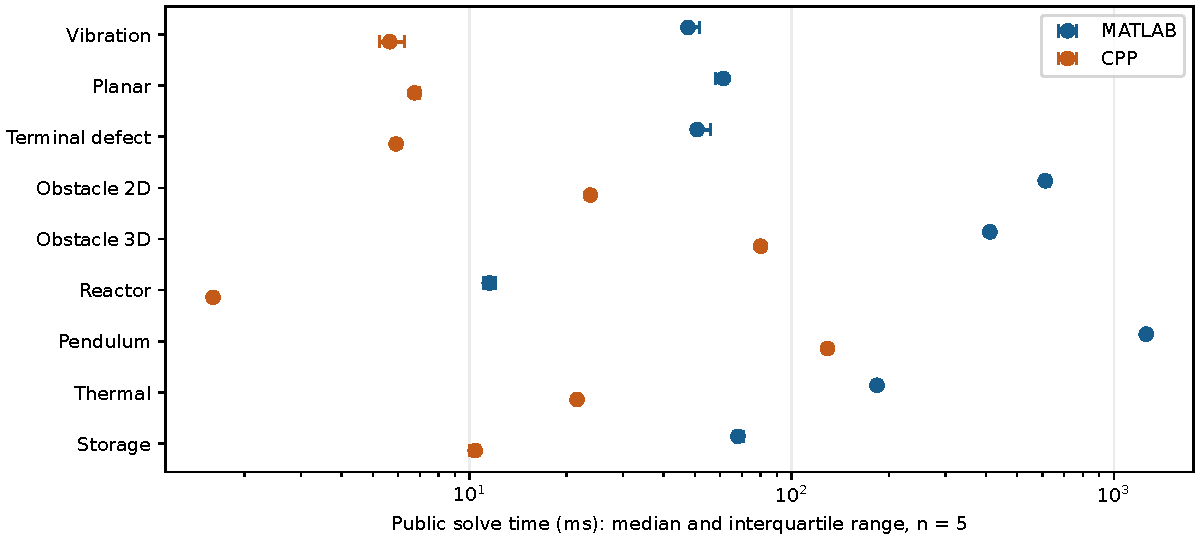
\includegraphics[width=\textwidth]{generated/timing.pdf}
\caption{本机完整接口耗时。点为中位数，横线为四分位区间；横轴为对数坐标。}
\end{figure}
\begin{figure}[H]
\centering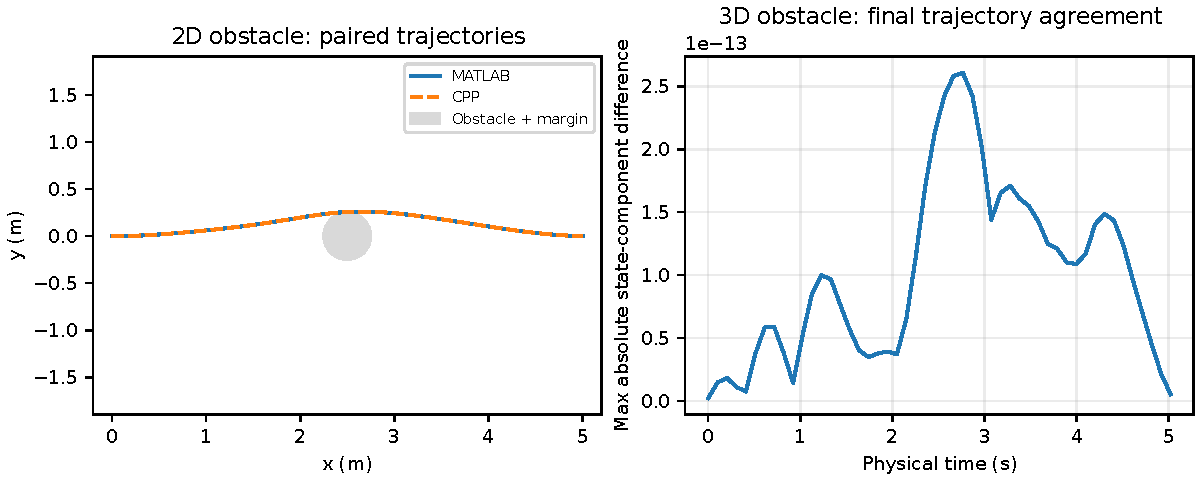
\includegraphics[width=\textwidth]{generated/trajectory_agreement.pdf}
\caption{左：二维避障轨迹重合；灰色区域为障碍物与物理安全裕度。右：三维案例各节点的最大绝对状态分量差，核对重启阶段输出的一致性。}
\end{figure}

九例的两种语言均通过各自的物理验收；Euler 一致性缺陷为浮点舍入量级。独立 RK4 缺陷并不等于零，它反映当前 Euler 网格相对于更高精度积分的误差，不能由较小的跨语言差异替代。九例完整轨迹高度一致；新二维、三维避障的最大状态分量差分别约 $4.80\times10^{-14}$ 和 $2.61\times10^{-13}$，活动控制差约 $2.09\times10^{-13}$ 和 $8.50\times10^{-13}$。两例均通过原终端误差、控制界、精确线段净空与独立积分检查。

CTest 对所有九例最终状态和活动控制使用统一的 $2\times10^{-6}$ 归一化阈值，不再对三维最终轨迹放宽容差。主迭代首轮检查 $10^{-9}$ 误差；终端缺陷及几何分支的全部实际 merit 试探记录和历史另以 $10^{-8}$ 检查。确定性重启阶段的候选记录和下降历史使用 $10^{-8}$，最终返回目标使用 $10^{-9}$。这些是当前九例的回归契约，不是任意问题的逐步等价证明。

\section{结果解释}
运行时间比值描述记录机器上完整实现的综合差异；五次重复与单台机器不能证明普遍性能优势。
MATLAB 与原生 C++ 的接口范围以本章和头文件为准。局部离散检查不等于全程连续模型验证。

\subsection{解析回放的双语言验收}
MATLAB 与 C++ 均对支持的恒速几何模型检查解析零阶保持回放。
结果字段分别为 \code{analytic_zoh_clearance_lower_bound} 和
\code{analytic_zoh_terminal_error}；前者必须非负，后者必须满足终端容差。
二者是独立于 Euler 节点的模型验证，不是算法全局最优性证明。
正式轨迹主图只展示当前解，双语言表继续比较相同输入下的 MATLAB 与 C++。


\chapter{自动测试与验证指标}

\section{测试分层}

\begin{longtable}{p{0.21\textwidth}p{0.69\textwidth}}
\toprule
层级 & 主要内容\\
\midrule
\endhead
单元测试 &
算法 ID 唯一性、旧名称映射、约束符号、输入校验、保存/加载、状态转移导数、时间重建、三维 clearance、线段穿障检测、缺陷定位和隐藏绘图。\\
集成测试 &
六个稳定算法及正式轨迹、热过程和储能示例的端到端运行。\\
回归测试 &
关键目标函数、终端误差、净空和运行结果保持在已记录范围内。\\
发布验证 &
干净副本中的示例、测试、元数据、许可证和命名范围检查。\\
\bottomrule
\end{longtable}

\section{数值稳定性与失败回滚}

六个维护算法不再显式求逆。控制方向的多个右端一起求解，先对称化
$H=(Q_{uu}+Q_{uu}^{\mathsf T})/2$，令 $s=\max(1,\|H\|_\infty)$。
最多尝试 12 个系统：先用原矩阵，再依次增加 $10^{-8}s$ 至 $10^2s$ 的对角阻尼。
候选系统必须正定，倒条件数估计至少为 $10^{-12}$，解及残差均需有限，并满足
\[
 \|(H+\lambda I)z-b\|_\infty\le
 10^{-10}\max(1,\|H+\lambda I\|_\infty\|z\|_\infty+\|b\|_\infty).
\]
MATLAB 使用反斜杠、C++ 使用带主元 LU 求解；Cholesky 用于正定性检查。
有阻尼时，价值递推也使用该控制 Hessian；所报告物理目标不变。
这不保证整个非线性问题凸化或全局收敛，模型仍需提供正确导数。

标量时间曲率为非有限值或绝对值小于 $10^{-18}$ 时停止，不能把零曲率变成虚构的时间方向。
原 Newton 公式允许的有限负曲率仍保留。航点算法原有 LM 正定性重试限制为每轮最多 80 次；
每次重试重置段索引及终端导数，只有预期的非正定性才触发重试。

更新前保存具有有限状态、控制、时间和目标的名义解。反向求解失败、控制或 rollout 非有限、
候选目标溢出时回滚到该解；惩罚分支返回其严格历史最优名义解。
如果初始化就没有有限名义解，直接抛出错误。
已知数值失败返回 \code{success=false} 和 \code{numerical_failure}；
模型回调的编程错误继续抛出，不会被伪装成数值停止。几何后处理不会覆盖致命数值失败。

\begin{description}[leftmargin=1.5em]
 \item[\code{converged}] 明确的停止规则与独立物理检查同时通过。
 \item[\code{feasible_not_converged}] 物理检查通过，但未满足求解器停止规则。
 \item[\code{numerical_failure}] 已知数值故障导致停止，诊断保留具体原因。
 \item[\code{failed_checks}] 返回解没有通过独立物理检查。
\end{description}
两个实现分别公开物理检查与停止规则的通过标志；有限轨迹、目标改善或迭代预算耗尽都不单独表示收敛。
代价变化停止也不等同于一阶驻点证明。旧 MATLAB 原始结果缺少停止字段时仍有兼容路径，六个维护算法均已显式报告停止信息。

诊断包含线性求解次数、正则化次数、最大阻尼、反向重试次数及失败原因。
测试覆盖奇异/不定/病态系统、非有限输入、时间奇异、预算耗尽、80 次重试上限、
非有限状态与目标溢出回滚，以及编程错误传播；没有放宽既有终端、净空或跨语言容差。
详细契约见 \code{docs/NUMERICAL_ROBUSTNESS.rst}。

\section{独立导数核对与模型回归}

离线接口 \code{ddpack.checkDerivatives} 和 C++ 的
\code{check_derivatives}。它们由使用者显式调用，不插入优化迭代。
函数值的维数、实数性与有限性先单独检查；不能仅因差分两侧有限就认为中心测试点有效。
对第 $j$ 个输入分量采用
\[
 \widehat D_{ij}=\frac{g_i(z+\delta_j e_j)-g_i(z-\delta_j e_j)}{2\delta_j},
 \qquad \delta_j=\epsilon\max(1,|z_j|).
\]
Hessian 由一阶梯度的中心差分核对，另检查混合导数的两个方向和对称性。
逐分量接受条件为
\[
 \frac{|D_{ij}-\widehat D_{ij}|}
 {10^{-7}+5\times10^{-6}\max(|D_{ij}|,|\widehat D_{ij}|)}\le1.
\]

MATLAB 核对所选算法的离散 Euler 状态/控制导数，以及适用的归一化时间导数、终端与运行代价导数、约束状态和控制梯度。
C++ 核对自主物理时间模型的动力学、代价和约束状态梯度；原生接口不提供独立时间或约束控制梯度回调，报告明确列出这些未覆盖项。

九个正式模型分别取三个非零状态/控制测试点，并使用 $10^{-4},10^{-5},10^{-6}$ 三个差分宽度，
每语言共 81 组。MATLAB 的 1755 项、C++ 的 1314 项检查均通过；这些计数包含函数值契约、导数差分和对称性检查。
最大容差比约 0.10842。两语言测试坐标逐项核对，不能把原生物理时间导数与 MATLAB 离散时间矩阵的数值误差直接当作同量纲比较。

反例检测错误导数、维数错误、非有限输出、回调异常和仅中心点无效的函数；
非可分双控制代价验证非零混合 Hessian。约束梯度在可行域内外均有测试。
\code{experiments/derivative_results} 保存每项记录、坐标和参数，Python 校验器核对 162 个源码哈希；
重复记录、错误源码绑定和不一致坐标的反向测试均被拒绝。

\begin{lstlisting}
p = ddpack.problems.linearRegulation();
r = ddpack.checkDerivatives(p,[0.3;-0.2],0.15, ...
    'Algorithm','free_time_pddp', ...
    'TimeScale',1.7,'IntegrationStep',0.037);
disp(struct2table(r.checks));
assert(r.success);
\end{lstlisting}

这是指定点与差分宽度下的局部数值一致性检查，不证明全域导数正确、物理模型正确或优化器收敛。
跨越非光滑点或模型定义域边界时应检查报告并调整测试点；没有核对裁剪、启发式修正、整个优化迭代或未使用的动力学二阶导数。
详细范围与复现命令见 \code{docs/DERIVATIVE_VALIDATION.rst}。

\section{运行代价检查与有限名义快照}
航点分支在完整累计目标后检查整条轨迹并保存名义快照，避免逐节点重复执行全轨迹扫描。
后续更新发生数值失败时，回退到已经完整验证的有限名义解。
当前九例双语言性能数据与复现方法见 \code{experiments/README.rst}；耗时只描述记录机器上的实现。

\section{成功判据}

统一结果只有同时满足以下条件才把 \code{success} 设为 true：
\begin{align}
  e_0 &\le \varepsilon_0,\\
  e_T &\le \varepsilon_T,\\
  v_{\mathrm{state}} &\le \varepsilon_G
  \quad\text{或该指标不适用},\\
  v_{\mathrm{control}} &\le \varepsilon_G,\\
  d_{\mathrm{Euler}} &\le \varepsilon_{\mathrm{dyn}},\\
  d_{\mathrm{RK4}} &\le \varepsilon_{\mathrm{RK4}}
  \quad\text{或仅报告},\\
  c_{\min} &\ge-\varepsilon_G
  \quad\text{或该指标不适用},\\
  J_{\mathrm{returned}}&\le J_{\mathrm{initial}}(1+10^{-10})
  \quad\text{当要求代价下降时}.
\end{align}

此外还要求所有数值有限、矩阵维度正确、时间严格递增，且底层求解器没有返回错误标志。
状态约束覆盖所有节点（含终点），终点使用最后一个有效保持控制。
对于 $G(x,u,\Delta t)=\Delta t\,g(x,u)$ 的阶段接口，验收使用 $G(x,u,1)$，避免小步长掩盖物理违反量。
约束输出必须为非空、有限实数向量，各节点分量数一致；回调异常保留原始原因。
不同物理量的尺度仍由模型作者选择，统一容差不自动完成量纲归一化。

Euler 和 RK4 必须完成全部区间诊断；\code{complete}、已完成与预期区间数、失败区间及异常标识/消息保存在 \code{metadata.defect_diagnostics}。
未计算项保留 NaN，含缺失项的最大缺陷为 $\infty$，不能用前缀的有限值代替全程最大值。
即使 RK4 容差设为 $\infty$，诊断异常也使 \code{success=false}。反例和复现命令见 \code{docs/ACCEPTANCE_VALIDATION.rst}。

这些局部诊断不等价于从初始状态出发的全程连续模型回放。
摆和热过程的独立名义回放曾超过终端容差，离散求解成功不能据此推断连续终点满足要求；连续应用需独立回放并细化重求。
当前材料不提供覆盖任意初值、目标、障碍和网格的稳健性结论。

航点和自由时间 PDDP 在预算退出时也重新计算返回轨迹的目标；\code{objective} 与 \code{raw.returned_cost} 对应实际状态、控制和物理时间。
迭代历史保留原记录，最后一项可能与预算退出后的目标不同；最后更新的目标溢出时回退到完整有限名义解并报告数值失败。
代价验收比较返回目标和原始初值目标，不用两项历史代价替代。

自定义 \code{minimum_time}/\code{maximum_time} 仅由二维、三维几何算法支持；其余四个算法收到这些参数会明确拒绝。
几何默认范围为 $[\max(T_0-20,5),T_0+7]$ s，需与用户提供的单边界共同满足次序要求；自由时间射击仍要求显式提供双边界。
验收再次检查实际返回时长，\code{time_bound_violation} 以秒报告超界量；即使求解器报告收敛，超界也不能成功。
三项修复的策略、反例与复现命令见 \code{docs/RETURN_REFINEMENT_TIME.rst}。

\section{已有测试证据}

当前代码的完整测试运行记录为
\[
  100\ \text{项测试},\qquad
  100\ \text{项通过},\qquad
  0\ \text{项失败}.
\]
2026-11-16 的正式验证中，九个正式示例、100 项 MATLAB 测试和八组 CTest 通过；其中含 11 项约束与诊断验收测试及 14 项返回目标、细化策略与时间边界测试。
C++ 已从发行源码编译，并通过对应反例；导数审计重新运行并通过 3069 项检查。
几何主阶段可停止于无下降方向，最终可行解依赖显式启用的射击阶段。

\code{TestDocumentation.m} 检查本 LaTeX 源文件、PDF、六个稳定算法 ID、正式运行命令及仓库首页。仓库首页采用官方模板要求的 \code{README.md}，并保留扩展说明 \code{README.rst}；

\chapter{结果查看与故障排查}

\section{输出文件}

每个正式示例通常生成：

\begin{longtable}{p{0.28\textwidth}p{0.60\textwidth}}
\toprule
文件 & 用途\\
\midrule
\endhead
\code{trajectory.png/pdf} & 轨迹、状态、控制和收敛图。\\
\code{summary.txt} & 人类可读的单算例结果摘要。\\
\code{metrics.csv/json} & 成功标志、终端误差、约束违反、缺陷、净空和运行时间。\\
\code{defect_diagnostics.csv/json} & 每个时间步和状态分量的动力学缺陷。\\
\code{solution.mat} & 统一结果结构。\\
\code{config.json} & 示例、算法、随机种子、模型说明和单位。\\
\code{environment.txt} & DDPACK、MATLAB、系统和时间戳。\\
\code{run.log} & 底层求解器输出。\\
\bottomrule
\end{longtable}

\section{重新加载和绘图}

\begin{lstlisting}
solution = ddpack.load( ...
    fullfile(resultFolder, 'solution.mat'));

disp(solution.success)
disp(solution.objective)
disp(solution.terminal_error)
disp(solution.metadata.metrics)

ddpack.plot(solution)
\end{lstlisting}

\section{常见问题}

\begin{description}[style=nextline,leftmargin=2em]
  \item[\code{Undefined function or variable}]
  先把 \code{tools} 加入路径，再运行
  \code{setup_ddpack('IncludeExamples',true)}。

  \item[\code{failed_checks}]
  不要只看底层 solver error。依次检查
  \code{terminal_error}、控制/状态违反量、Euler 缺陷、RK4 缺陷、净空和代价下降。
  \item[\code{feasible_not_converged}]
  独立数值检查已通过，但底层求解器明确报告尚未收敛，例如达到最大迭代次数。可以把轨迹描述为“数值可行”，但不能写成“算法收敛”；应增加迭代、重新缩放模型或启用有记录的终端投影后再验证。

  \item[输出目录已存在]
  DDPACK 为保护证据拒绝覆盖。更换新目录或不传
  \code{OutputDir}，让程序自动生成时间戳目录。

  \item[无界面环境绘图失败]
  使用 \code{Visible=false}，并确认 MATLAB 能创建不可见 figure 且输出目录可写。

  \item[几何算法返回正净空是否等于安全证明]
  不是。它只说明离散轨迹线段对指定圆/球的数值 clearance 为正。

  \item[旧名称警告]
  把 \code{pddp}、\code{c_pddp}、\code{mspddp}、
  \code{cbf_mspddp_*}、\code{fft_cddp}
  替换为当前公共 ID。
\end{description}

\chapter{自定义问题开发清单}

\section{建模步骤}

\begin{enumerate}[leftmargin=2.4em]
  \item 明确每个状态和控制的物理意义、单位和维数。
  \item 实现连续动力学 \code{F}。
  \item 实现所选算法需要的
  \code{Phi}、\code{beta/Beta}、\code{theta/gamma}。
  \item 实现代价及一阶、二阶导数。
  \item 把所有约束统一为 $G\ge0$ 可行。
  \item 设置具有物理意义的终端误差、约束、Euler 和 RK4 容差。
  \item 先用 \code{QuickMode=true} 做冒烟测试。
  \item 检查状态、控制、代价、缺陷和约束，而不是只看一张轨迹图。
  \item 固定随机种子并保存配置、环境和结果。
\end{enumerate}

\section{线性模型模板}

对于
\[
  \dot{\bm{x}}=A\bm{x}+B\bm{u}+\bm{b},
\]
可直接使用：

\begin{lstlisting}
problem = struct();
problem.name = 'my_linear_problem';
problem.x0 = [1; 0];
problem.xf = [0; 0];
problem.tf = 15;
problem.dt = 0.3;
problem.dynamics = PointMassDynamics(A, B, drift);
problem.cost = QuadraticCost(Qf, Qs, R);
problem.u_max = umax;
problem.terminal_tolerance = 0.01;

options = ddpack.Options( ...
    'Algorithm', 'free_time_pddp', ...
    'MaxIterations', 80);

solution = ddpack.solve(problem, options);
\end{lstlisting}

\section{发布或论文使用注意}

\begin{itemize}[leftmargin=2em]
  \item 报告完整公共算法名和 ID，不只写历史缩写。
  \item 使用“实现变体”“受某理论结构启发”等准确表述。
  \item 不把 \code{terminal_defect_pddp} 宣称为完整多重射击。
  \item 不把几何修正算法宣称为标准 Lie 导数 CBF 或形式化安全证明。
  \item 不把 \code{penalty_free_time_ddp} 宣称为 FFT 算法或完整增广 Lagrangian 方法。
  \item 同时报告终端误差、动力学缺陷、约束违反和净空，而不是只报告目标函数。
\end{itemize}

\backmatter

\chapter*{附录 A：算法 ID 速查}
\addcontentsline{toc}{chapter}{附录 A：算法 ID 速查}

\begin{longtable}{p{0.31\textwidth}p{0.21\textwidth}p{0.36\textwidth}}
\toprule
公共 ID & 旧名称 & 最适合的已验证任务\\
\midrule
\endhead
\code{free_time_pddp} & \code{pddp} & 线性/振动调节，单标量自由时间。\\
\code{waypoint_pddp} & \code{c_pddp} & 航点、倒立摆、二维点质量。\\
\code{terminal_defect_pddp} & \code{mspddp} & 三状态曲线机动。\\
\code{geometric_safety_pddp_2d} & \code{cbf_mspddp_2d} & 二维圆形障碍物。\\
\code{geometric_safety_pddp_3d} & \code{cbf_mspddp_3d} & 三维球形障碍物。\\
\code{penalty_free_time_ddp} & \code{fft_cddp} & 反应器、热过程、储能和状态下界。\\
\bottomrule
\end{longtable}

\chapter*{附录 B：完整正式运行命令}
\addcontentsline{toc}{chapter}{附录 B：完整正式运行命令}

\begin{lstlisting}
repo = 'path/to/DDPACK';
addpath(fullfile(repo, 'tools'));
setup_ddpack('IncludeExamples', true);

summary = run_publication_examples( ...
    'Visible', false, ...
    'QuickMode', false);

benchmark = run_benchmarks;
results = run_all_tests;
\end{lstlisting}

\vfill
\begin{center}
\color{gray}
本说明书依据 DDPACK 1.1.0 候选代码实现整理。\\
代码行为、公共注册表和独立数值诊断优先于历史名称与早期注释。
\end{center}

\end{document}
